\documentclass[11pt,a4paper,headinclude,footinclude,chapterprefix=on]{scrreprt} 
\usepackage[utf8]{inputenc} 
\usepackage[T1]{fontenc} 
\usepackage{tabularx} 
\usepackage{multicol} 
\usepackage{graphicx} 
\usepackage{tikz} 
\usepackage{amssymb} 
\usepackage{textcomp} 
\usepackage{longtable}
\usepackage{hyperref}


% ================================================================
% Variables
% ================================================================
\newcommand{\trnumber}{TKN-14} 
\newcommand{\trdate}{March 2014} 
\newcommand{\trauthor}{Aravinth, Sivalingam Panchadcharam} 
\newcommand{\tremail}{me@aravinth.info} 
\newcommand{\trtitle}{Variations in WiFi RSSI values due to different types of Interferences}

% ================================================================
% Page Style
% ================================================================
\usepackage{geometry} \geometry{a4paper, inner=30mm, outer=25mm, top=40mm, bottom=42mm}

\usepackage[headsepline,plainheadsepline,footsepline,plainfootsepline]{scrpage2} \clearscrheadfoot

\ihead[\Large {\scshape TU Berlin }]{\Large {\scshape TU Berlin }}

\ifoot[{\tiny 
\begin{minipage}
	{4.0cm}Copyright at Technical University Berlin. 
	\newline All Rights reserved. 
\end{minipage}
}]{{\tiny 
\begin{minipage}
	{4.0cm}Copyright at Technical University Berlin. 
	\newline All Rights reserved. 
\end{minipage}
}} \cfoot[\scriptsize \trnumber]{\scriptsize \trnumber} \ofoot[Page 
\pagemark]{Page 
\pagemark}

\pagestyle{scrheadings}

\usepackage{mathptmx} 
\usepackage[scaled=.92]{helvet} 
\usepackage{courier}

\addtokomafont{pagefoot}{\normalfont}

% ================================================================
% Start of Document
% ================================================================
\begin{document} 
\bibliographystyle{plain}

% ================================================================
% Cover Sheet
% ================================================================
{ \sffamily

\thispagestyle{empty} 
\begin{tabularx}
	{\columnwidth}{cXc} 
	
\includegraphics[height=1cm]{Images/TU-Logo-3D-rot.pdf} & & 
	
\includegraphics[height=1cm]{Images/tknlogo.pdf} \\
\end{tabularx}

\vspace{1.0cm} 
\begin{center}
	{\huge 
	\noindent Technical University Berlin
	
	\vspace{0.5cm}
	
	\noindent Telecommunication Networks Group 
	\begin{center}
		\rule{15.5cm}{0.4pt} 
	\end{center}
	} 
\end{center}
\begin{minipage}
	[][11.0cm][c]{14.5cm} {\Huge 
	\begin{center}
		\trtitle 
	\end{center}
	\begin{center}
		\trauthor \\
		{\Large \tremail} 
	\end{center}
	\begin{center}
		Berlin, \trdate 
	\end{center}
	
	\vspace{0.5cm}
	
	} 
\end{minipage}

\setlength{\fboxrule}{0.4pt} \setlength{\fboxsep}{0.4pt} 
\begin{center}
	
	\rule{15.5cm}{0.4pt}
	
	\vspace{0.5cm}
	
	{\huge {Project in advanced network technologies}}
	
	\vspace{0.5cm}
	
	{\huge Supervisors: Filip Lemic, Dr. Arash Behboodi}
	
	\vspace{0.5cm} 
\end{center}
}

% ================================================================
% Abstract
% ================================================================
\begin{abstract}
\subsection*{\abstractname} WiFi Beacon packets are transmitted periodically to announce the presence of WiFi. Beacon Packet RSSI is Received Signal Strength Indicator which indicates the power of signal that is received at the receiver. RSSI is used by networking interface card to determine the energy level in the channel. However, RSSI values are extensively used for ranging and localization purpose where accuracy and reliability should be guaranteed \cite{ref:rssi}. However, previous studies predict that RSSI values changes due to change in distance and various interferences. In oder to analyze whether there is a variation in RSSI values due to different type of interferences, we have designed a reference scenario and two interference scenarios. Experiments were conducted and repeated. It yielded large set of data. In oder to process and analyze the raw data, a visualization tool was implemented. Processed data was analyzed and statistical results were plotted. Finally, It shows that variations in RSSI values due to interferences. Furthermore, It is recommended to conduct more experiments to get significant results with additional help of the work done in this project.

\subsection*{Keywords} RSSI, WiFi beacon, interferences, indoor localization

\subsection*{Acknowledgment} Filip Lemic, Dr. Arash Behboodi, TKN, Technical University of Berlin
\end{abstract}

% ================================================================
% Tableofcontents
% ================================================================
\tableofcontents

% ================================================================
% Introduction
% ================================================================
\chapter{Introduction} 
\section{Beacon Packet} In Wireless Local Area Network Beacon Packets are transmitted periodically by Base Station Set (BSS) to announce the presence of WiFi Network. Beacon Packet is one of the management frames in IEEE 802.11. Figure \ref {fig:beacon} shows the fields of Beacon Packet. Beacon interval expressed in Time Unit (TU). It is a configurable parameter in the AP and typically configured as 100 TU. 
\begin{figure}
	[!h] \centering 
	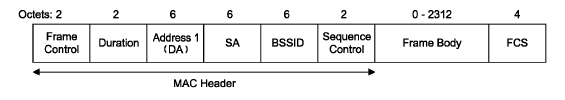
\includegraphics[width=15cm]{Images/beacon_frame.png} \caption{MPDU - Beacon Packet of IEEE 802.11} \label{fig:beacon} 
\end{figure}

\section{Received Signal Strength Indicator (RSSI)} RSSI is an indication of the power level received by a receiver expressed in dBm. RSSI is defined as ten times the logarithm of the ratio of power of the received signal and a reference power (e.g., 1mW). RSSI is used by networking interface card (NIC) to determine the amount of radio energy in the channel.


\section{RSSI in Indoor Localization} RSSI is also extensively used for RF based ranging and localization purposes. RSSI is defined as ten times the logarithm of the ratio of power of the received signal and a reference power. It is known that power dissipates from a point source as it moves further out and the relationship between power and distance is that power is inversely proportional to the square of the distance traveled. In this way the distance from the sender to receiver can be calculated for localization purpose.

\section{Accuracy} Different studies \cite{ref:wifi:chipset} show that RSSI values have significant variations due to various factors. 
\begin{itemize}
	\item RSSI values are reported significantly different by different hardwares. 
	\item RSSI values vary with change in temperature. 
	\item RSSI values are affected by various interferences. 
	\item The relation between RSSI values and distance between transmitter and receiver is unreliable. 
\end{itemize}
\begin{figure}
	[!h] \centering 
	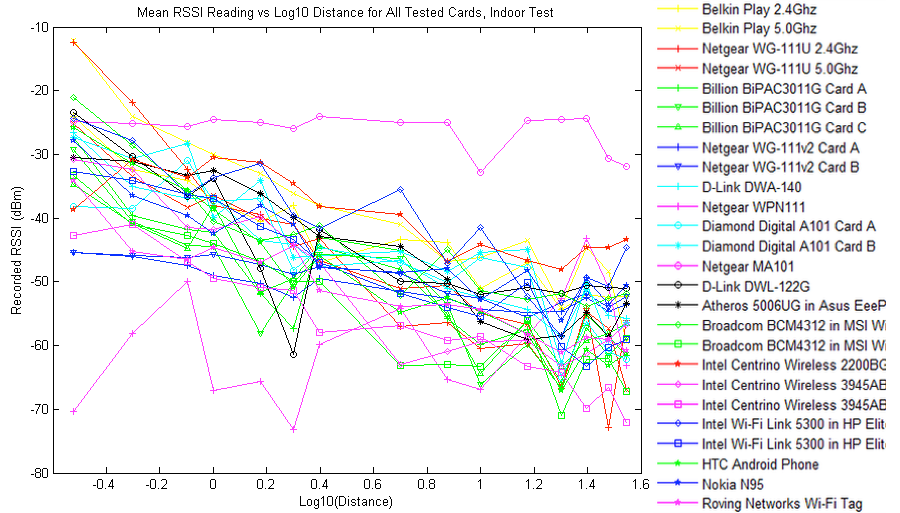
\includegraphics[width=13cm]{Images/rssi_vendor1.png} \caption{RSSI values recorded from different hardwares} \label{fig:rssi_vendors} 
\end{figure}

\section{Standardization} There is no standardized relationship of any particular physical parameter to the RSSI reading. The 802.11 standard does not define any relationship between RSSI value and power level in mW or dBm. Vendors and chipset makers provide their own accuracy, granularity, and range for the actual power (measured as mW or dBm) and their range of RSSI values (from 0 to RSSI Max). Figure \ref{fig:rssi_vendors} shows the variance of RSSI values due to different hardwares and vendors.

\section{Interferences} It is known that power dissipates from a point source as it moves further out and the relationship between power and distance. This power is inversely proportional to the square of the distance traveled. However, previous experimental studies show that RSSI values could be influenced by various interferences such as data traffic in the same channel, full power transmissions or jamming signals, architectural obstructions causing reflections and scattering.

\section{Motivation} RSSI is also used for other purposes where accuracy and reliability should be guaranteed. From previous studies, it was predicted that RSSI values are influenced by interferences in the wireless spectrum.

\section{Solution} This explains the process of our work during this project. 
\begin{itemize}
	\item Previously completed works were studied. It includes mainly EVARILOS Project which was implemented to benchmark various RF based indoor localization algorithm. 
	\item Knowledge about experiment infrastructure was obtained. It includes testbed, robot for automation, tools, networking devices, signal generators and interference sources. 
	\item Previously collected measurement data was obtained. It was achieved by retrieving data from R2DM (Raw Ranging Data Management). 
	\item Experiments were designed. It includes the selection of appropriate interference parameters. 
	\item Implementation of Raw Ranging Data Visualization Tool. Significant amount of work in this project was done to implement this tool since it is used to visualize the larger data sets which were obtained during the experiments. 
	\item Experiments were carried out in 3 difference scenarios. The data obtained was visualized and the experiments were repeated. 
	\item Data was processed using Visualization tool, analyzed statistically to plot graphs and results were obtained. 
	\item Report was written. It contains detailed information about the whole project and obtained results. 
\end{itemize}

% ================================================================
% Design
% ================================================================
\chapter{Design} 
\section{Reference Scenario}\label{scene:ref} This reference scenario is instantiated on the 2nd floor of the TWIST testbed. It is called “Reference scenario” because no artificial interference is generated and the presence of uncontrolled interference is minimized. According to the EVARILOS Benchmarking Handbook (EBH), this scenario is an instance of the “Small office” type of scenarios. In this scenario 20 measurement points are defined and their locations are given in Figure \ref{fig:floor}. 
\begin{figure}
	[!h] \centering 
	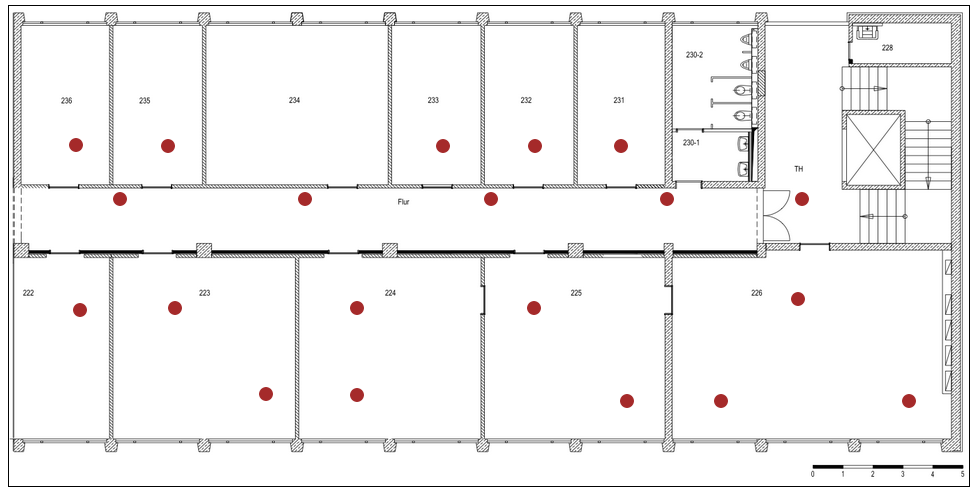
\includegraphics[width=100mm]{Images/floor} \caption{Locations of measurement points} \label{fig:floor} 
\end{figure}

\paragraph{} At each measurement point the indoor localization System Under Test (SUT) is requested to estimate location. The SUT device is carried to each measurement location using the robotic platform. The navigation stack of the robotic platform gives one order of magnitude more accurate location estimation than considered SUTs and the location obtained from the robotic platform is considered as the ground truth.

\paragraph{} The experiments were performed at the weekend afternoon, so the influence of interferes has been minimized. Furthermore, the wireless spectrum has been measured using the WiSpy device attached to the robotic platform and all measurements with the interference threshold above certain level have been repeated. Finally, before each experiment a more detailed measurement of the spectrum has been taken with the spectrum analyzer at a predefined location.

\section{Interference Scenarios}\label{sec:interference} 
\subsection{Interference Scenario 1 - Jamming}\label{scene:int:1} First interference scenario instantiated in TWIST testbed uses the testbed Wireless Fidelity (WiFi) nodes as interference sources. Interference type is jamming on one IEEE 802.11 channel with the maximum transmission power. The jamming node is located at one location in the testbed environment for interference scenario 1. Summary of this interference scenario is given in Table \ref{tb:interf:1}. 
\begin{table}
	[h] \centering \caption{Interference scenario 1} \label{tb:interf:1} 
	\begin{tabular}
		{|l|l|} \hline \multicolumn{2}{|c|}{Types of interference sources} \\
		\hline WiFi & \checkmark \\
		Microwave & \texttimes \\
		DECT & \texttimes \\
		Bluetooth & \texttimes \\
		3G & \texttimes \\
		ZigBee & \texttimes \\
		\hline \multicolumn{2}{|c|}{Types of interference sources} \\
		\hline Number of sources & 1 \\
		Power & 20 dBm \\
		Waveform & Carrier jamming \\
		Specific pattern & \\
		Start \& stop time & Beginning \& end of experiment \\
		Traffic model & \\
		\hline 
	\end{tabular}
\end{table}

\subsection{Interference Scenario 2 - Data Traffic}\label{scene:int:2} 
Second interference scenario instantiated in TWIST testbed defines interference types that is usual for the office and home environments. Namely, interference is emulated using 4 WiFi embedded Personal Computers (PCs), namely a server, email client, data client, and video client. The server acts as a WiFi Access Point (AP) and a gateway for the emulated services. The email client will “check email” once every 15 seconds for a duration of one second. The data client is emulated via TCP streams one starting at 45 seconds for a duration of 22.5 seconds and the other starting at 105 seconds for a duration of 45 seconds. The video client is emulated as a UDP stream of 100 kbps for half the experiment cycle and it will start at the middle of the experiment. In total, the experiment takes 150 seconds. Summary of this interference scenario is given in Table \ref{tb:interf:3}. 
\begin{table}
	[h] \centering \caption{Interference scenario 2} \label{tb:interf:3} 
	\begin{tabular}
		{|l|l|} \hline \multicolumn{2}{|c|}{Types of interference sources} \\
		\hline WiFi & \checkmark \\
		Microwave & \texttimes \\
		DECT & \texttimes \\
		Bluetooth & \texttimes \\
		3G & \texttimes \\
		ZigBee & \texttimes \\
		\hline \multicolumn{2}{|c|}{Types of interference sources} \\
		\hline Number of sources & 3 \\
		Power & 20 dBm \\
		Waveform & \\
		Specific pattern & \\
		Start \& stop time & Beginning \& end of experiment \\
		Traffic model & WiFi traffic \\
		\hline 
	\end{tabular}
\end{table}

% ================================================================
% RSSI Visualization Tool
% ================================================================
\chapter{Raw Ranging Data Visualization Tool} 
\section*{Introduction} Measurements yield large amount of raw data which contains the complete information of experiments such as testbed measurement locations, access points, rssi, channel, ssid, bssid, latency. In order to track collected raw data, a raw ranging data visualization tool was implemented. 

\paragraph{}This tools helps us to list and visualize the available databases and collections of experiments under one hood. It is a web-based standalone software which was implemented using Javascript and various libraries. This tool can be simply started by opening it on a web browser. It needs an Internet connection to retrieve data from the backend servers. It makes use of asynchronous (AJAX) ability of Javascript and processes large array of raw data. This tool consists of 4 panels which showcases the work flow in an user friendly manner. Usage and functionality of each panel is explained in the following sections. 
\begin{figure}
	[!h] \centering 
	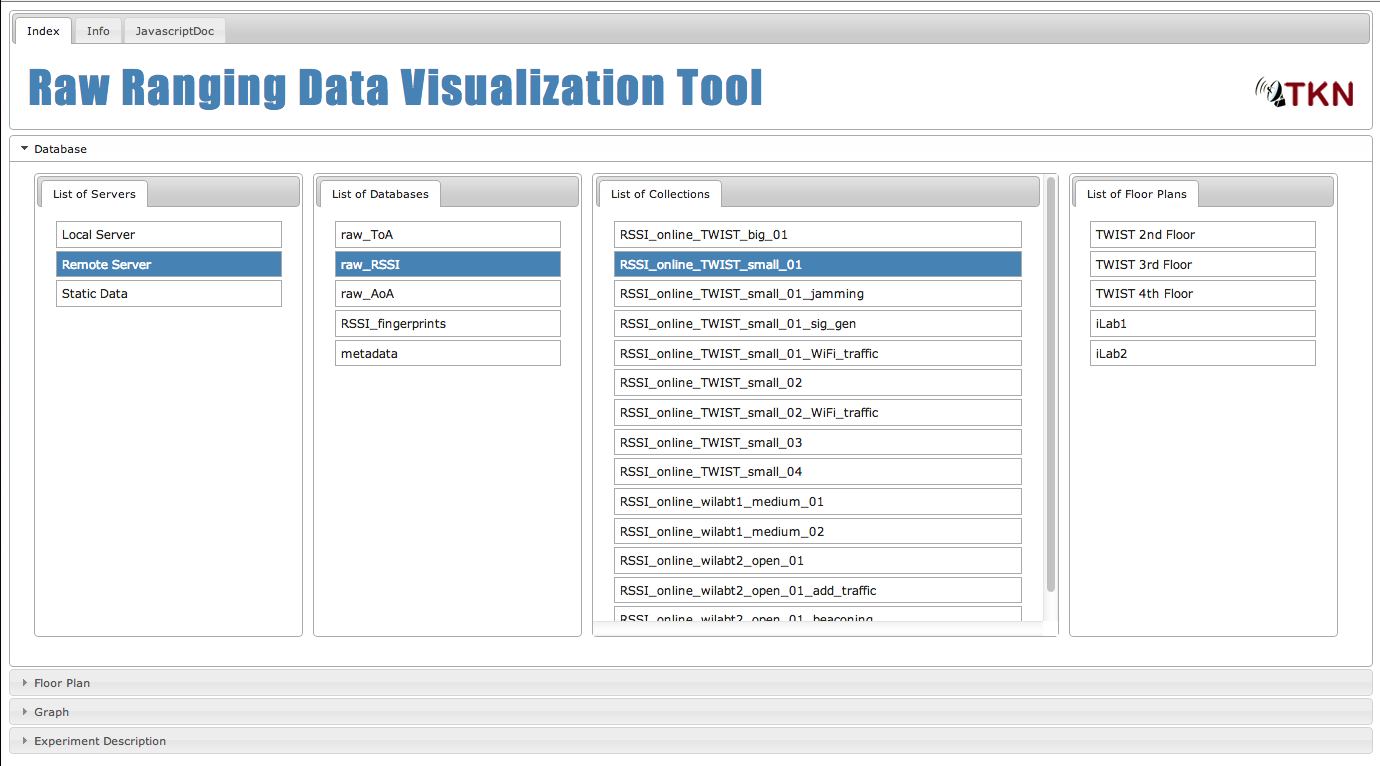
\includegraphics[width=13cm]{Images/tool_db.png} \caption{Dashboard of the visualization tool} \label{fig:tool:db} 
\end{figure}

\section{Dashboard} Figure \ref{fig:tool:db} shows the Dashboard panel that is the landing page of this tool. It contains 4 sub-panels. 
\begin{description}
	\item[List of Servers] lists URIs of server that contains various RAW data collected from the experiments. Remote Server contains the complete set of RAW data. Copy of the RAW data can also be stored on the local machine. Static Data contains a simple set of RAW data for the purpose of debugging. 
	\item[List of Databases] lists URIs of databases which are stored in the server. 
	\item[List of Collections] lists the collections of experiments which were carried out. URI denotes the name of Testbed, experiment size and experiment type. 
	\item[List of Floor Plans] lists the names of the floor plans on which experiments were carried out. Floor Plan must be selected according to the experiment. 
\end{description}
\begin{figure}
	[!h] \centering 
	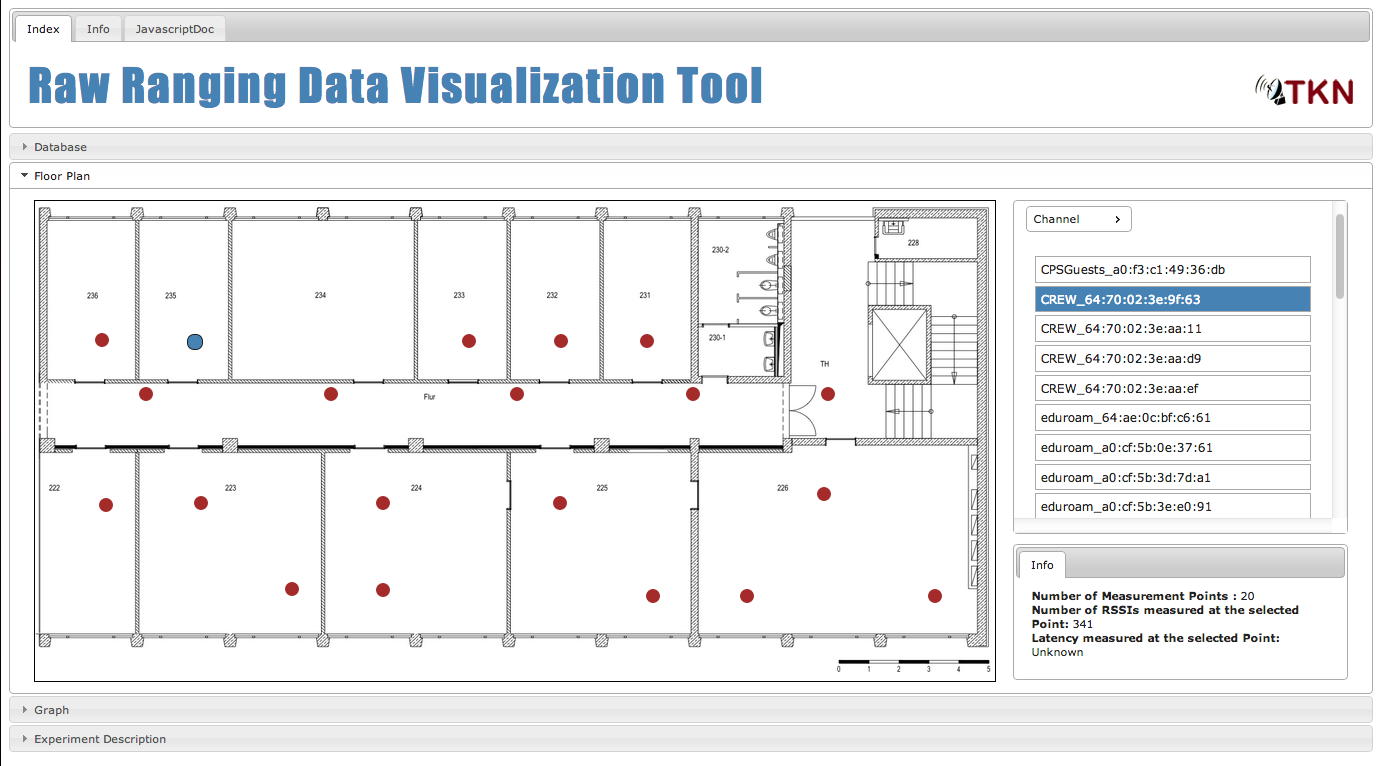
\includegraphics[width=13cm]{Images/tool_floor.png} \caption{Floor Plan of the visualization tool} \label{fig:tool:floor} 
\end{figure}

\section{Floor Plan} Figure \ref{fig:tool:floor} shows Floor Plan panel that contains the map of selected testbed. Once the appropriate floor plan for an experiment is selected, all the measurement points are loaded into the map. Measurement point is circular button that turns blue when it is clicked and it lists RSSI values measured at that geographical point. On the right side of the Floor Plan, Channel and SSID information of the selected measurement point is shown. If the Raw Data contains channel information, then it will be listed in the dropdown other it will be listed as Unknown. RSSI values are grouped together on the basis of same SSID and BSSID. Info tab at the right below shows some specific information about the selected measurement point. 
\begin{figure}
	[!h] \centering 
	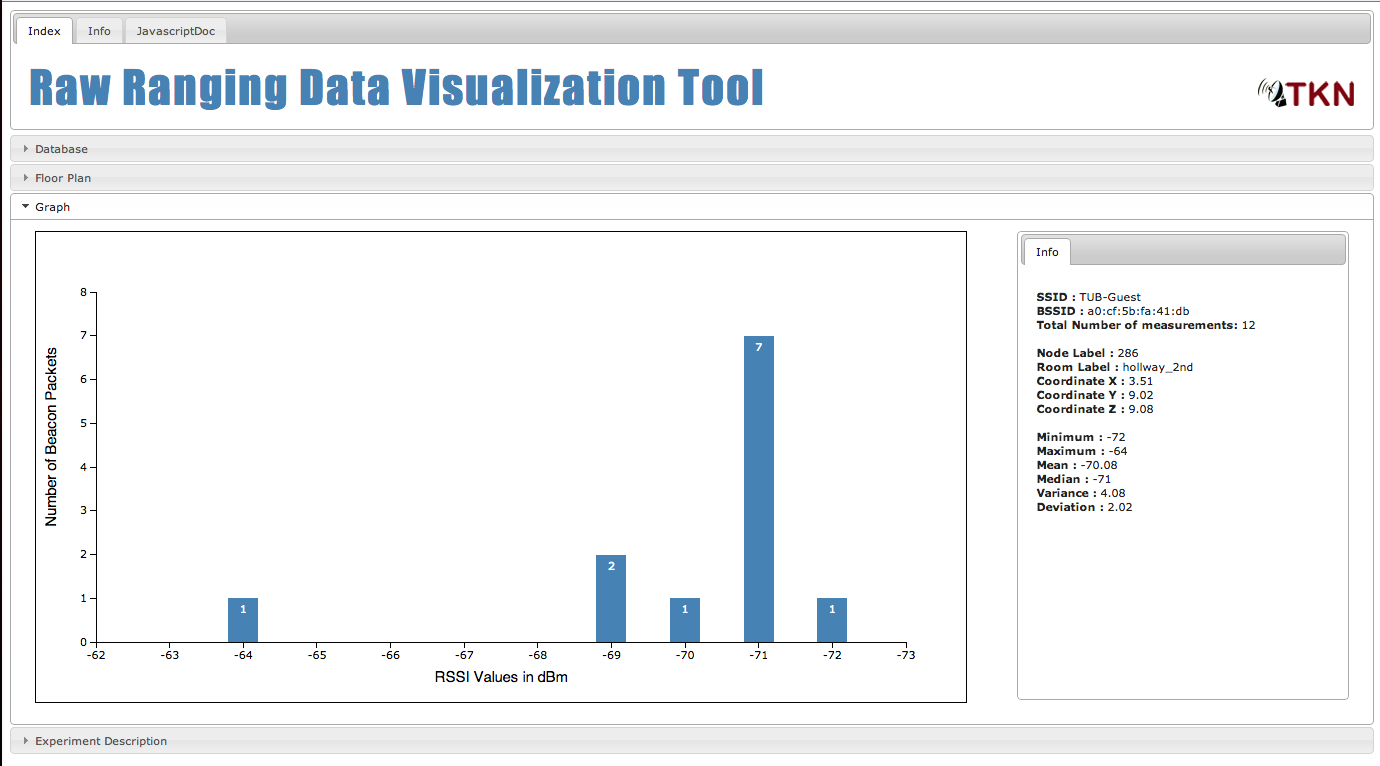
\includegraphics[width=13cm]{Images/tool_graph.png} \caption{Graph of the visualization tool} \label{fig:tool:graph} 
\end{figure}

\section{Graph} Figure \ref{fig:tool:graph} shows Graph panel that contains a histogram that is generated dynamically by selecting a particular access point on Floor Plan panel. Number of Bins of the histogram are also dynamically adjusted based on the total number of RSSI values measured. Info tab shows coordinate information of the selected measurement points as well as the statistics of RSSI values. 
\begin{figure}
	[!h] \centering 
	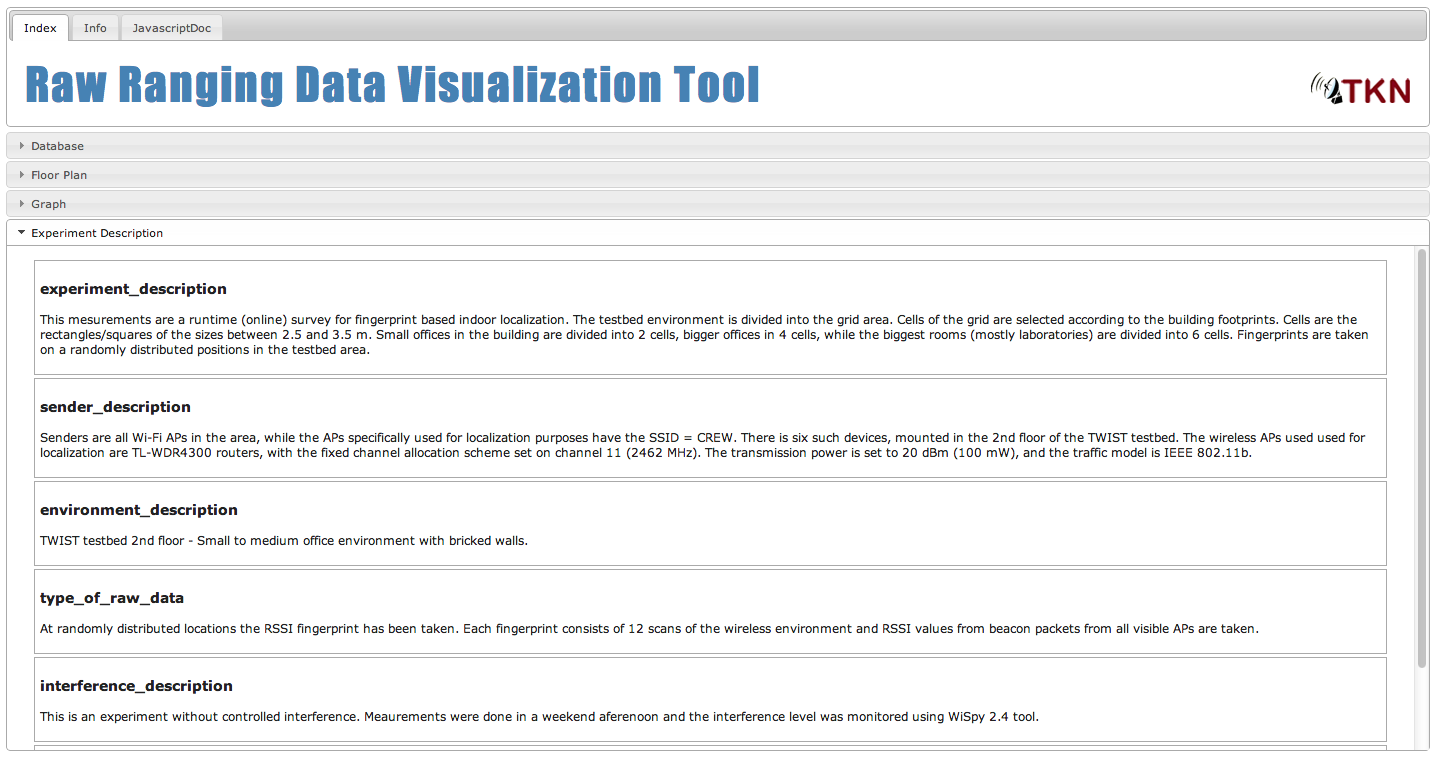
\includegraphics[width=13cm]{Images/tool_des.png} \caption{Experiment Description of the visualization tool} \label{fig:tool:des} 
\end{figure}

\section{Experiment Description} Figure \ref{fig:tool:des} shows Experiment Description panel that contains detail of the experiment such as testbed environment, sender and receiver device specification and interference pattern. This information is stored in Metadata database. 
\begin{figure}
	[!h] \centering 
	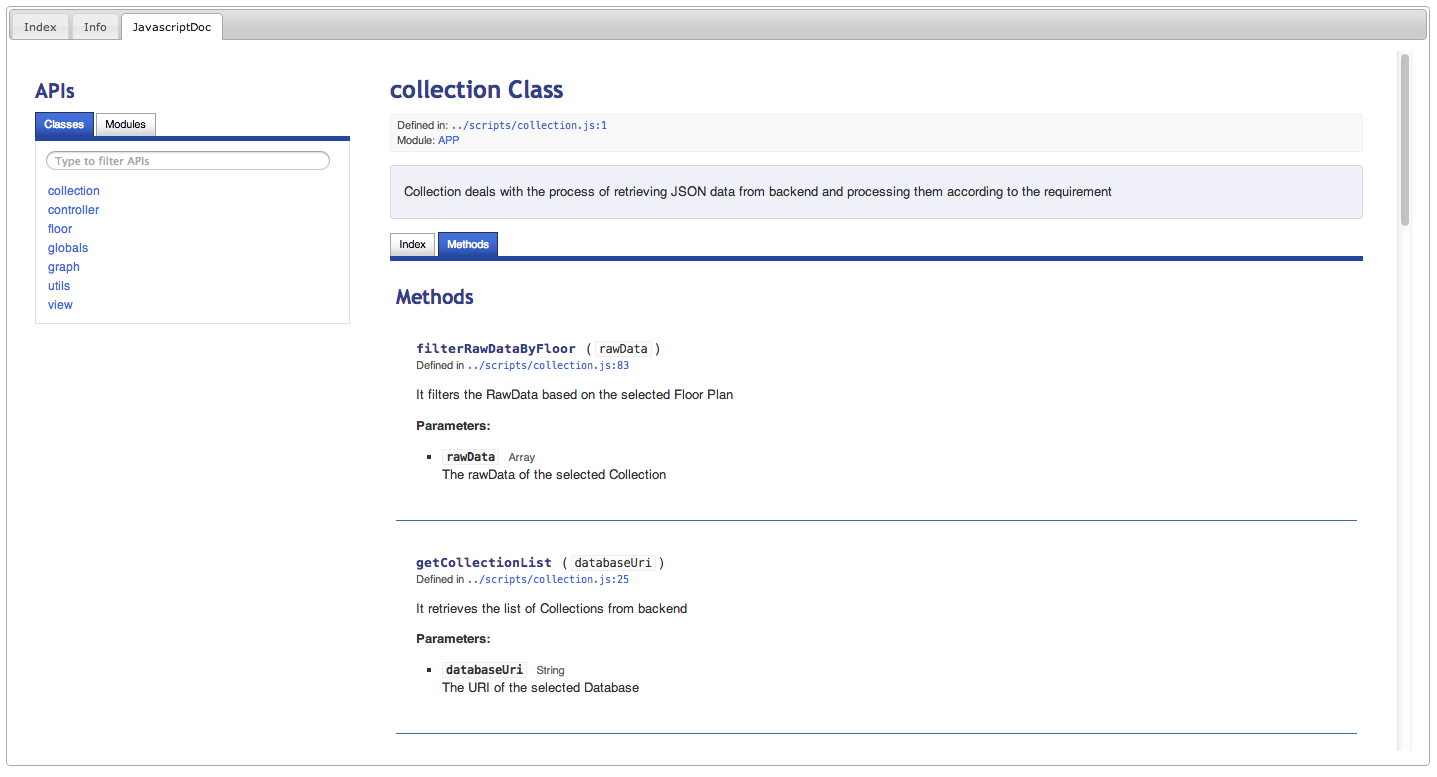
\includegraphics[width=13cm]{Images/tool_jsDoc.png} \caption{API of the visualization tool} \label{fig:tool:jsDoc} 
\end{figure}

\section{API} Figure \ref{fig:tool:jsDoc} shows API that is a Javascript documentation which can be viewed by clicking on JavascriptDoc button on the top menu. API reveals the Functions, Constants, Views, Collections, Events and Utilities used to visualize the Raw Ranging Data. It helps to extend this program, do further implementation, add new features and debug the code. 

\section{Source Code}
Source code of this project is maintained in an online repository.  The repository contains also the documents, presentations, scripts, tools, images, etc have been used in this project. It can be found in \url{https://github.com/AravinthPanch/rssi}.




% ================================================================
% Experiments
% ================================================================
\chapter{Experiments} 
\section{Infrastructure} Experiments are carried on a testbed \cite{ref:crew}. As shown in the figure \ref{fig:experiment}, Testbeds provide a robotic automated platform to carry out the experiment. Setting up the measurement points, configuring the nodes, accessing signal generators and various other devices are done with the help of control center. 
\begin{figure}
	[!h] \centering 
	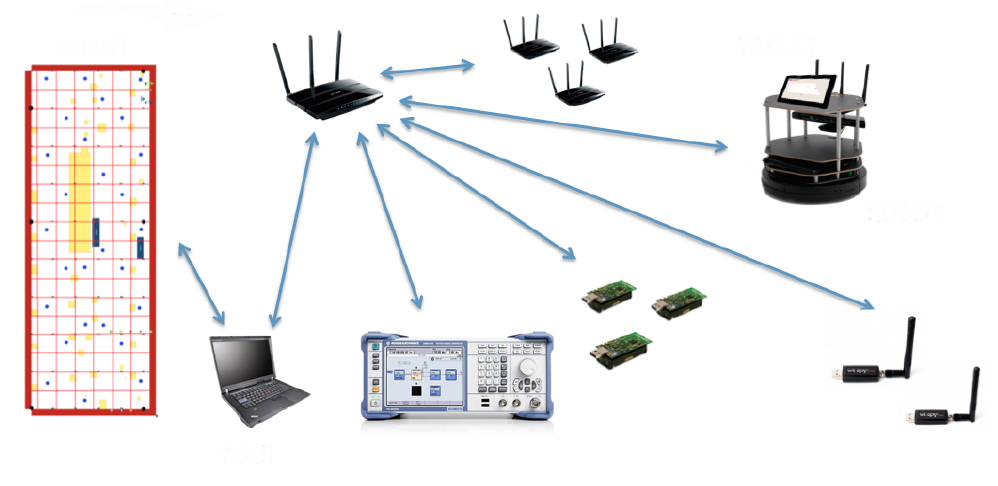
\includegraphics[width=13cm]{Images/evari.png} \caption{Experiment Environment} \label{fig:experiment} 
\end{figure}

\section{Testbed} 
\subsection{TWIST} The TKN Wireless Indoor Sensor network Testbed (TWIST)  \cite{ref:twist}, developed by the Telecommunication Networks Group (TKN) at the Technische Universität Berlin, is a scalable and flexible testbed architecture for experimenting with wireless sensor network applications in an indoor setting. It provides basic services like node configuration, network-wide programming, out-of-band extraction of debug data and gathering of application data.

It is equipped with 102 TmoteSky nodes and 102 eyesIFX nodes. For the experiments 3 Different Floor Plans are used. Signal Generators are used to generate microwave signals which were used to jam the channel during the experiments. From control center fixed coordinates are set to the robot, so that accurate measurement points are achieved in the experiments. 

\section{Experiment Procedure} This shows step by step how experiments were carried out. 
\begin{itemize}
	\item Measurement points of testbed are loaded into the Robot. 
	\item System Under Test (SUT) is equipped with Network Interface Card (NIC) and loaded with program to store RSSI, SSID, BSSID, Latency values. 
	\item SUT is placed on the top of the Robot. 
	\item Robot is commanded from the control center to move to the first measurement point. 
	\item SUT is commanded to start the measurement. 
	\item SUT scans the Wireless Spectrum in the environment for WiFi Access Points and stores RSSI, SSID, BSSID, Latency values. This step is iterated 20 times. 
	\item Measurements are stored on cloud database. 
	\item Robot moves to other measurement point and repeats the above given steps 
\end{itemize}

\section{Reference Scenario Experiment} Since this experiment is conducted under environment where no artificial interference is generated and the presence of uncontrolled interference is minimized, this experiment is referred to as reference scenario. Experiments with controlled interferences are carried out in the similar way with artificially generated interferences. Section \ref{sec:interference} shows the details of various interferences which were generated during the experiments.

\subsection{Experiment Description} This measurements are a runtime (online) survey for fingerprint based indoor localization. The testbed environment is divided into the grid area. Cells of the grid are selected according to the building footprints. Cells are the rectangles/squares of the sizes between 2.5 and 3.5 m. Small offices in the building are divided into 2 cells, bigger offices in 4 cells, while the biggest rooms (mostly laboratories) are divided into 6 cells. Fingerprints are taken on a randomly distributed positions in the testbed area.

\subsection{Environment Description} TWIST testbed 2nd floor - Small to medium office environment with bricked walls.

\subsection{Sender Description} Senders are all WiFi APs in the area, while the APs specifically used for localization purposes have the SSID = CREW. There is four such devices, mounted on the corners of the 2nd floor of the TWIST testbed. The wireless APs used used for localization are TL-WDR4300 routers, with the fixed channel allocation scheme set on channel 11 (2462 MHz). The transmission power is set to 20 dBm (100 mW), and the traffic model is IEEE 802.11b.

\subsection{Receiver Description} Receiver is a MacBook Pro notebook with the AirPort Extreme network interface card (NIC).

\subsection{Raw Data} At randomly distributed locations the RSSI fingerprint has been taken. Each fingerprint consists of 20 scans of the wireless environment and RSSI values from beacon packets from all visible APs are taken.

\subsection{Interference Description} This is an experiment without controlled interference. Measurements were done in a weekend afternoon and the interference level was monitored using WiSpy 2.4 tool.

% ================================================================
% Analysis
% ================================================================
\chapter{Analysis} 
\section{Repeatability} \label{sec:repeat} \cite{ref:randr} \cite{ref:randr2}
\begin{equation}
	\label{eq:variance} {S}_i^2 = {\sigma}^2 = \frac{\sum\limits_{i=1}^{n} (x_{i} - \bar{X}^2)}{n-1} 
\end{equation}

In equation \ref{eq:variance}, $S_{i}^{2}$ is the variance of each cell, where each cell is test results of experiment that satisfies the repeatability condition, $(x_{i} - \bar{X}^2)$ is the difference from the mean value and $n$ is total number of values in the set. 
\begin{equation}
	\label{eq:repeat} {S}_r^2 = \frac{\sum\limits_{i=1}^{n} (n_{i} - 1){S}_i^2} {\sum\limits_{i=1}^{n}(n_{i} - 1)} 
\end{equation}

In equation \ref{eq:repeat}, ${S}_r^2$ is repeatability variance, n is total number of repetition of cell, $S_{i}^{2}$ is the variance of each cell. Therefore, Repeatability is simply the group variances of the test results.

\subsection{Repeatability Condition} It is defined as a condition where independent test s are obtained with the same method on identical test items in the same laboratory by the same operator using the same equipment within short intervals of time.

In our case, it is defined as a condition which satisfies the following: 
\begin{itemize}
	\item Same Testbed 
	\item Same Laboratory (Floor) 
	\item Same Measurement point 
	\item Same Channel 
	\item Same Sender (SSID and BSSID) 
\end{itemize}

An experiment which satisfies this condition is called as cell. 

% ================================================================
% Results
% ================================================================
\chapter{Results} From the data obtained, graphs between distance and mean of RSSI values, variance of RSSI values and group variances were plotted. From multiple experiments which were conducted with various interferences sources located at different location, the following graphs were obtained. The data is been grouped based on BSSID and analyzed. As learned from the previous experiments under environment with minimal interferences \cite{ref:rssi}, distance and RSSI show a linear relationship such that the RSSI value decreases with increase in distance. However, the experiments with various interference sources exhibit a non linear relationship of RSSI values with distance from the source and influenced significantly around the interference sources. These results show that there is variation in RSSI values due to interferences. The following sections show plotted graphs.

\pagebreak 
\section{Access Point : CREW 64:70:02:3e:9f:63} 
The details of the access point are given below.
\begin{itemize}
	\item SSID : CREW 
	\item BSSID : 64:70:02:3e:9f:63 
	\item Location : X-axis - 21.5m, Y-axis - 14.8m 
	\item Frequency : 2.4 GHz 
\end{itemize}
\subsection{Reference Scenario} 
Following plots show mean and variance of RSSI values from the access point (CREW 64:70:02:3e:9f:63). Mean and Variance are plotted spatially with color map to show the significance. As described in the section \ref{scene:ref}, these experiments were conducted in a scenario where no artificial interference is generated and the presence of uncontrolled interference is minimized.
\begin{longtable}
	{lr} 
	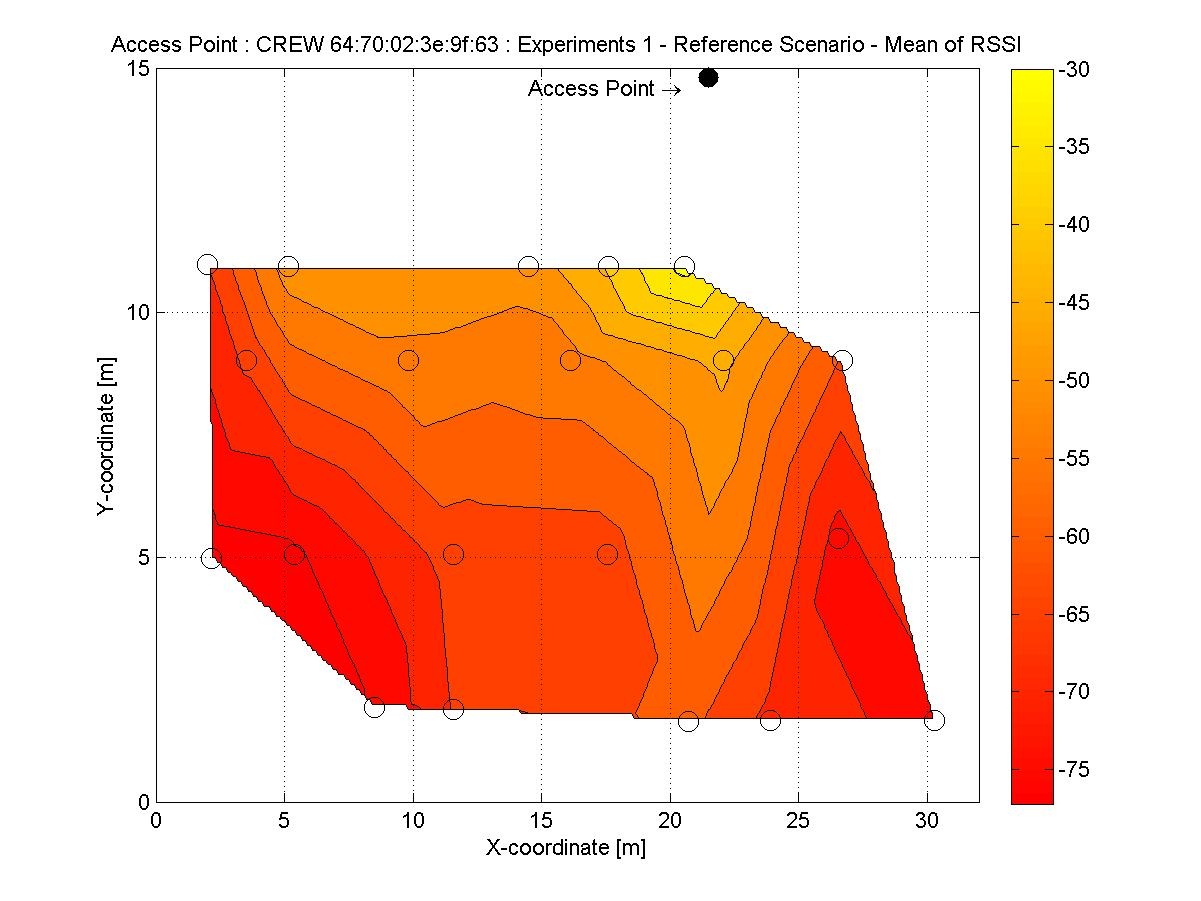
\includegraphics[width=13cm]{../../Source/plot/CREW_63/63_Ref_Ex_1_Mean.jpg} \\
	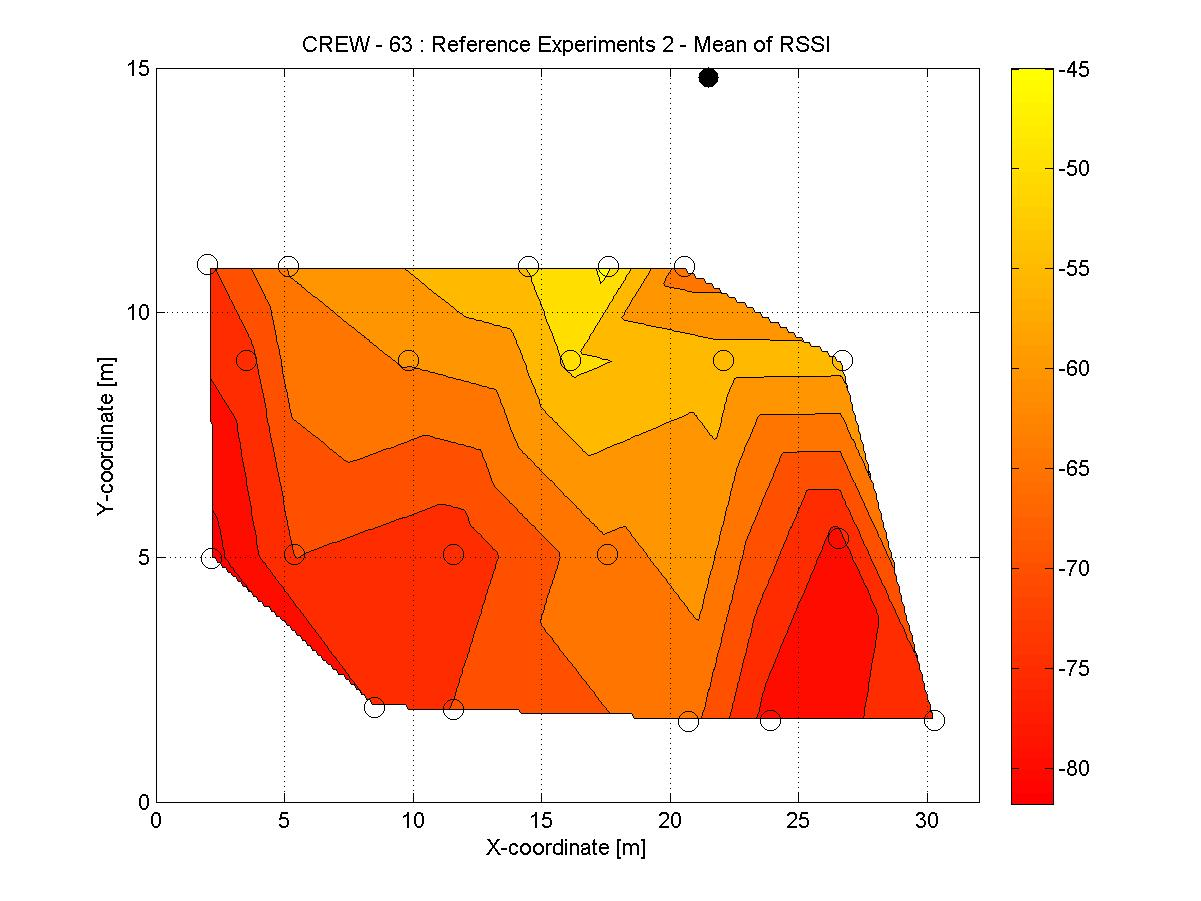
\includegraphics[width=13cm]{../../Source/plot/CREW_63/63_Ref_Ex_2_Mean.jpg} \\
	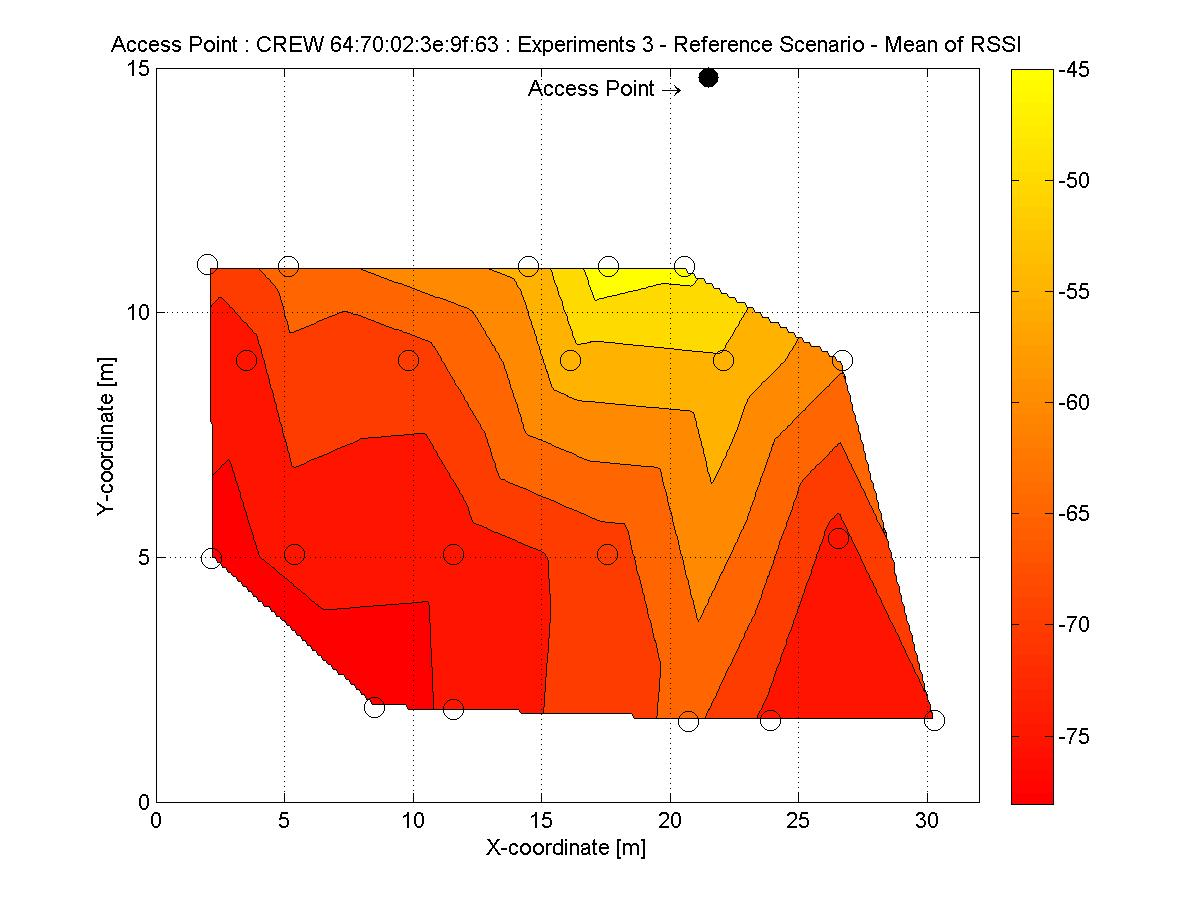
\includegraphics[width=13cm]{../../Source/plot/CREW_63/63_Ref_Ex_3_Mean.jpg} \\
	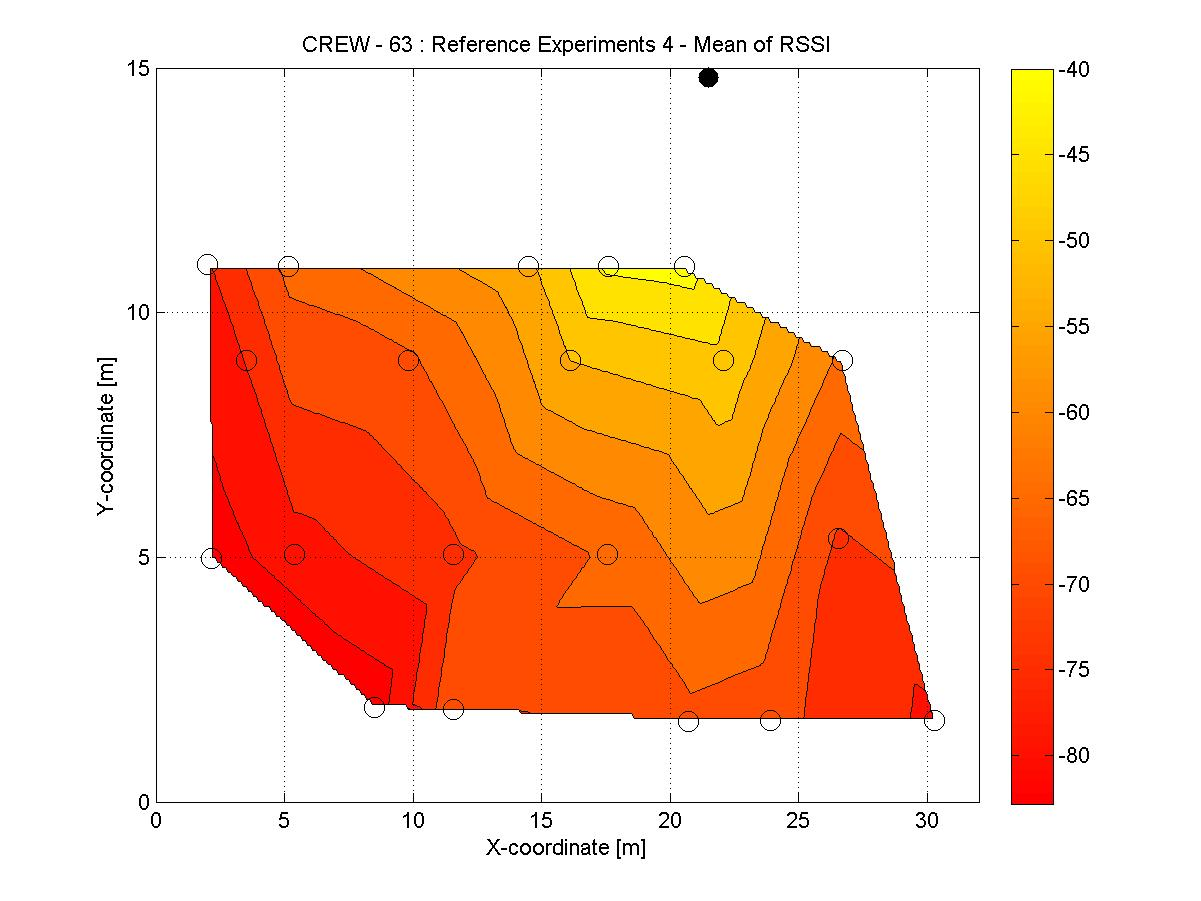
\includegraphics[width=13cm]{../../Source/plot/CREW_63/63_Ref_Ex_4_Mean.jpg} \\
	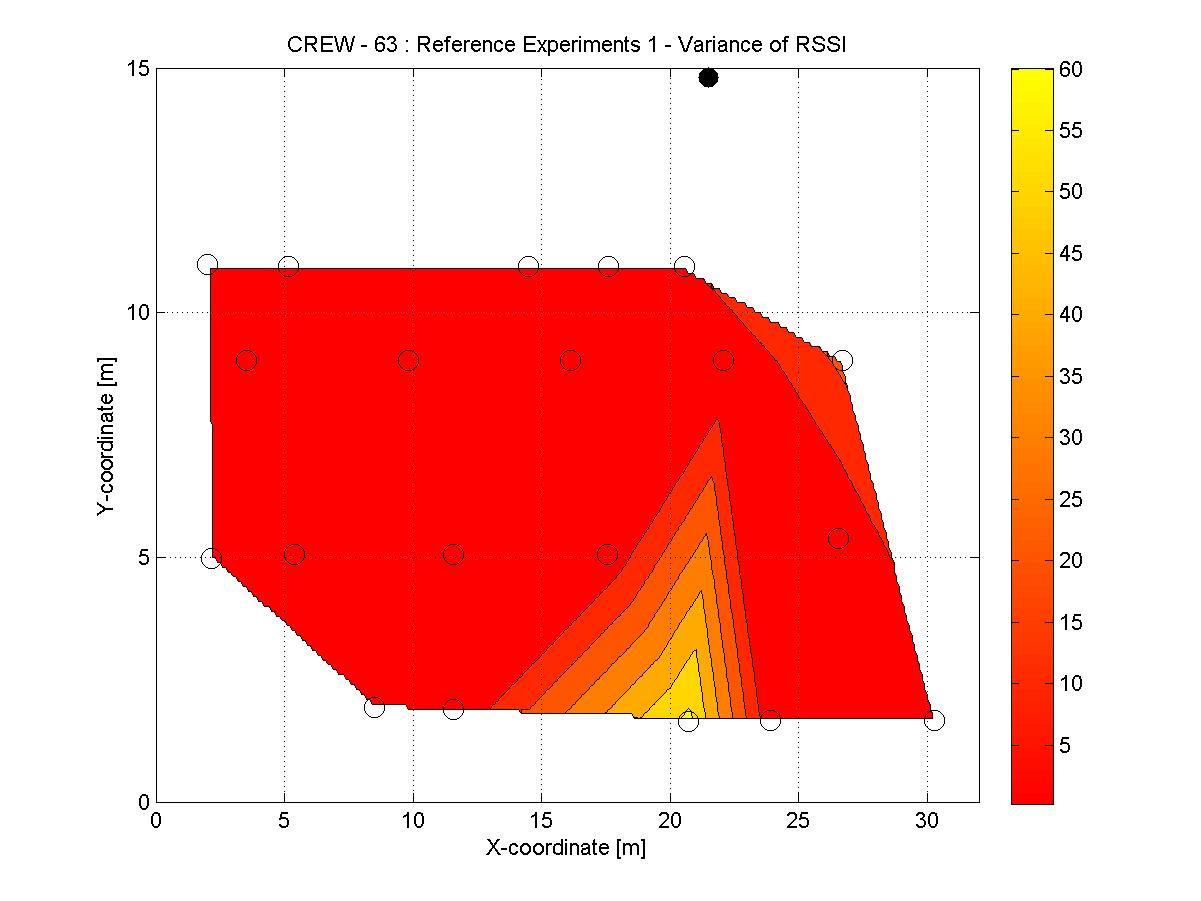
\includegraphics[width=13cm]{../../Source/plot/CREW_63/63_Ref_Ex_1_Variance.jpg} \\
	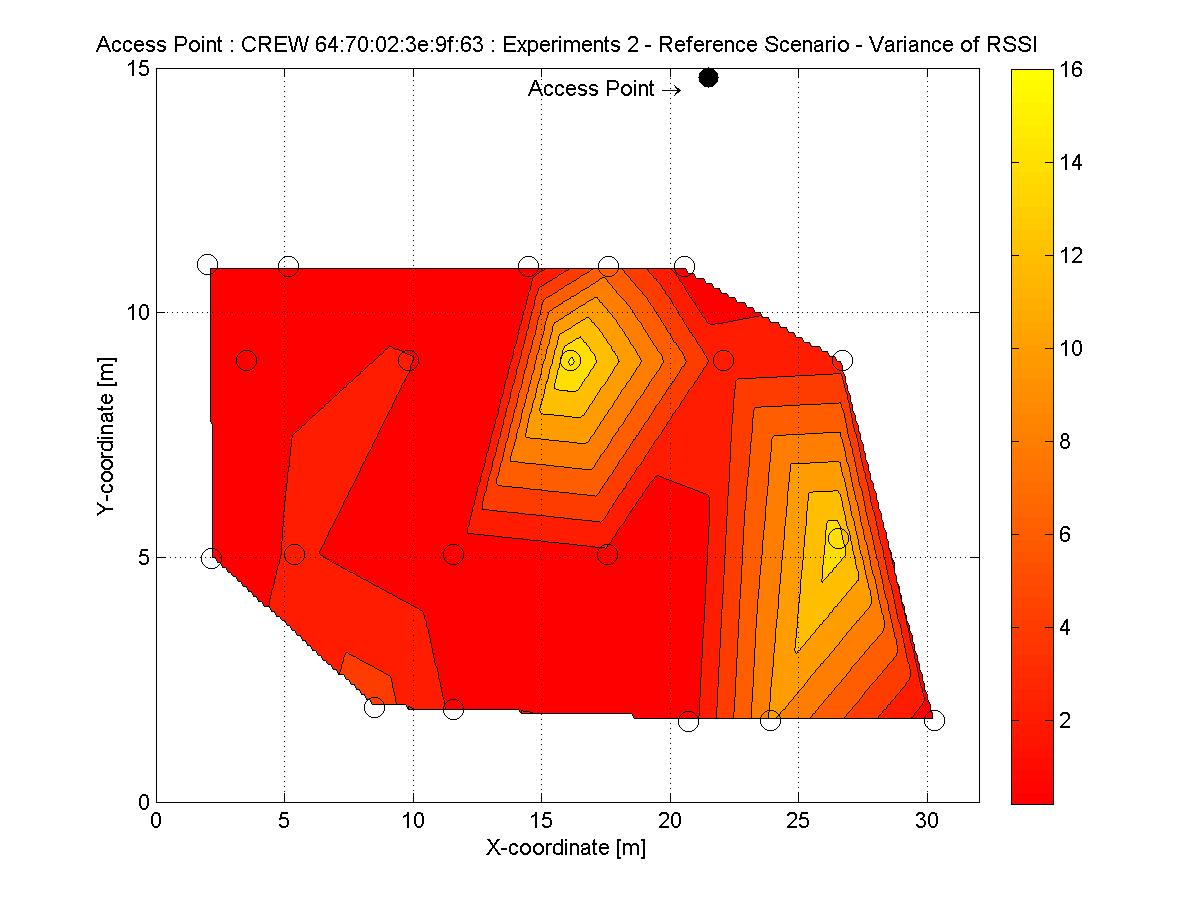
\includegraphics[width=13cm]{../../Source/plot/CREW_63/63_Ref_Ex_2_Variance.jpg} \\
	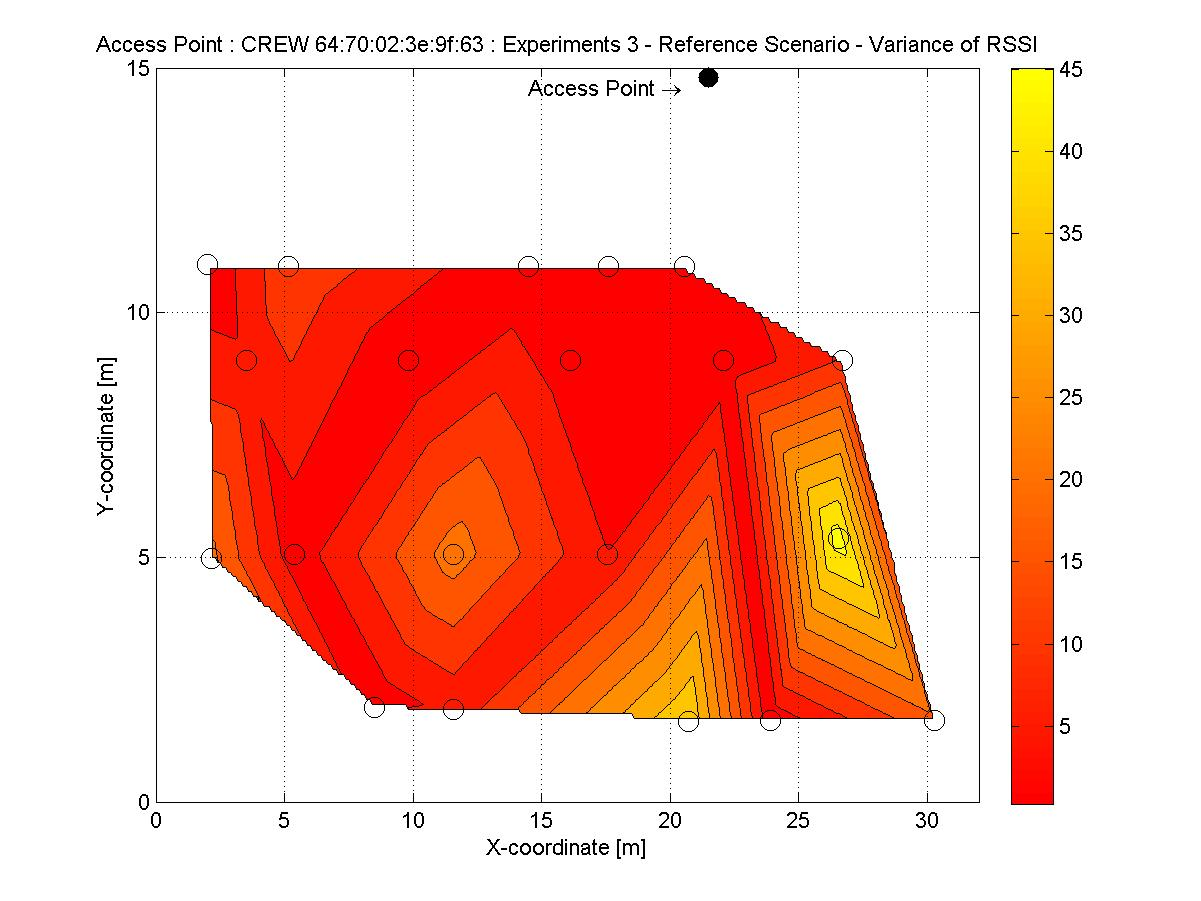
\includegraphics[width=13cm]{../../Source/plot/CREW_63/63_Ref_Ex_3_Variance.jpg} \\
	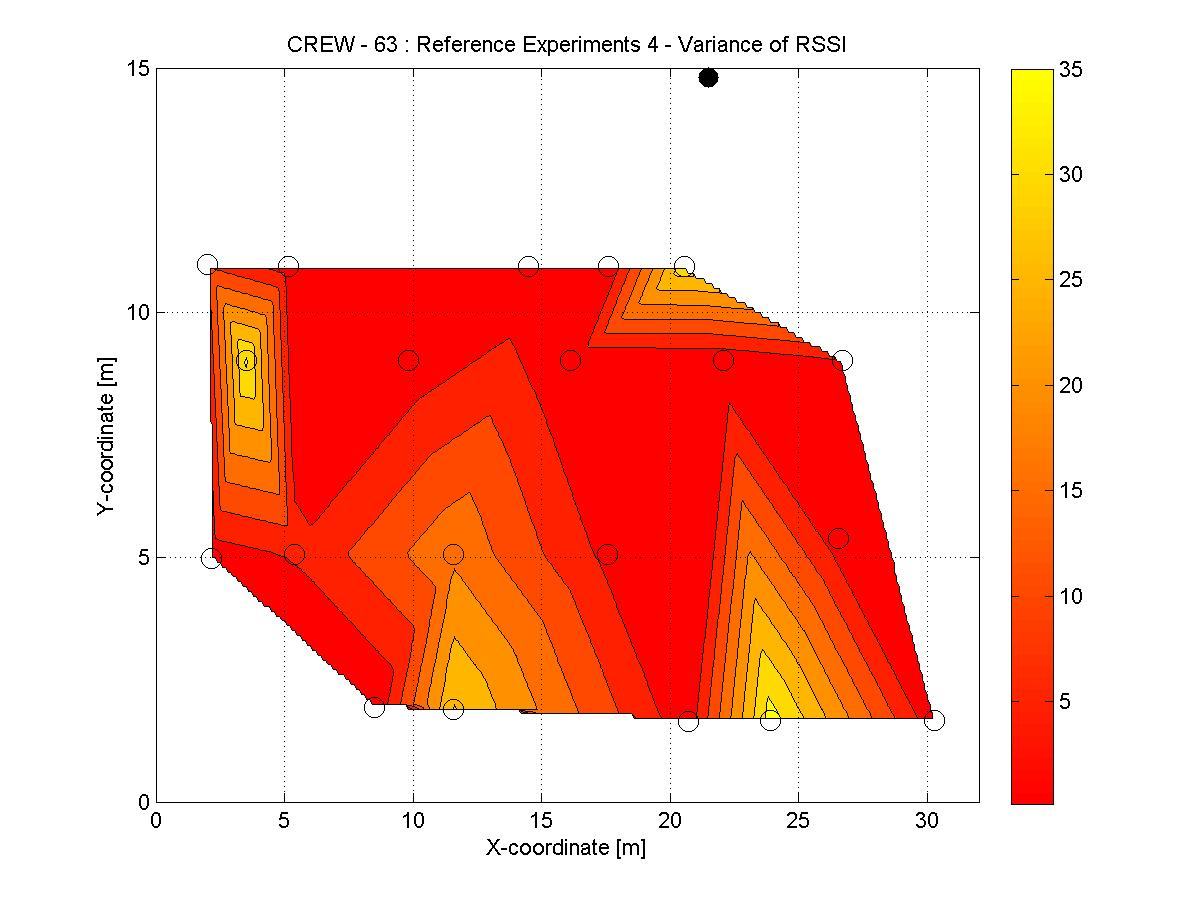
\includegraphics[width=13cm]{../../Source/plot/CREW_63/63_Ref_Ex_4_Variance.jpg} 
\end{longtable}

\subsection{Interference Scenario 1} 
Following plots show mean and variance of RSSI values from the access point (CREW 64:70:02:3e:9f:63). Mean and Variance are plotted spatially with color map to show the significance. As described in the section \ref{scene:int:1}, these experiments were conducted in a scenario where IEEE 802.11 channel was jammed with the maximum transmission power using signal generators.
\begin{longtable}
	{lr} 
	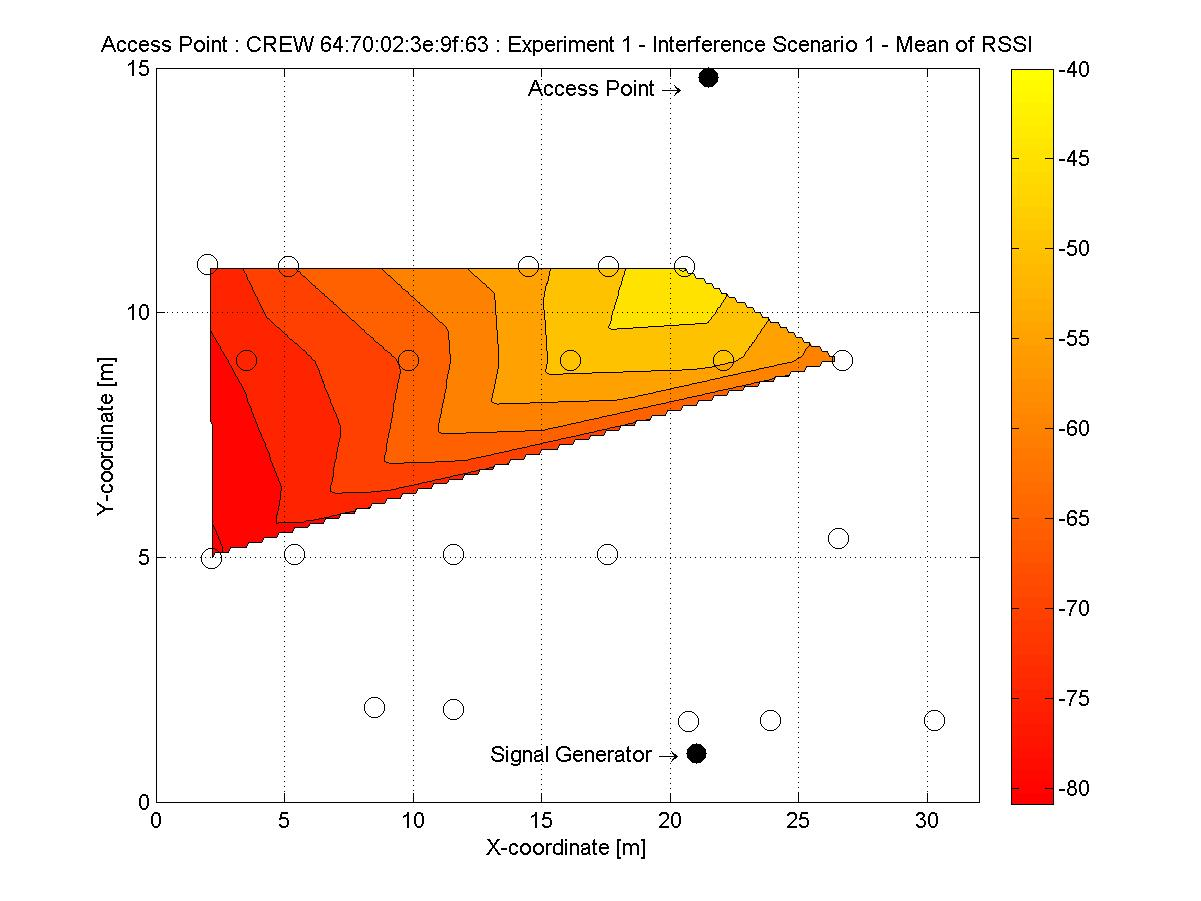
\includegraphics[width=13cm]{../../Source/plot/CREW_63/63_Sig_Ex_1_Mean.jpg} \\
	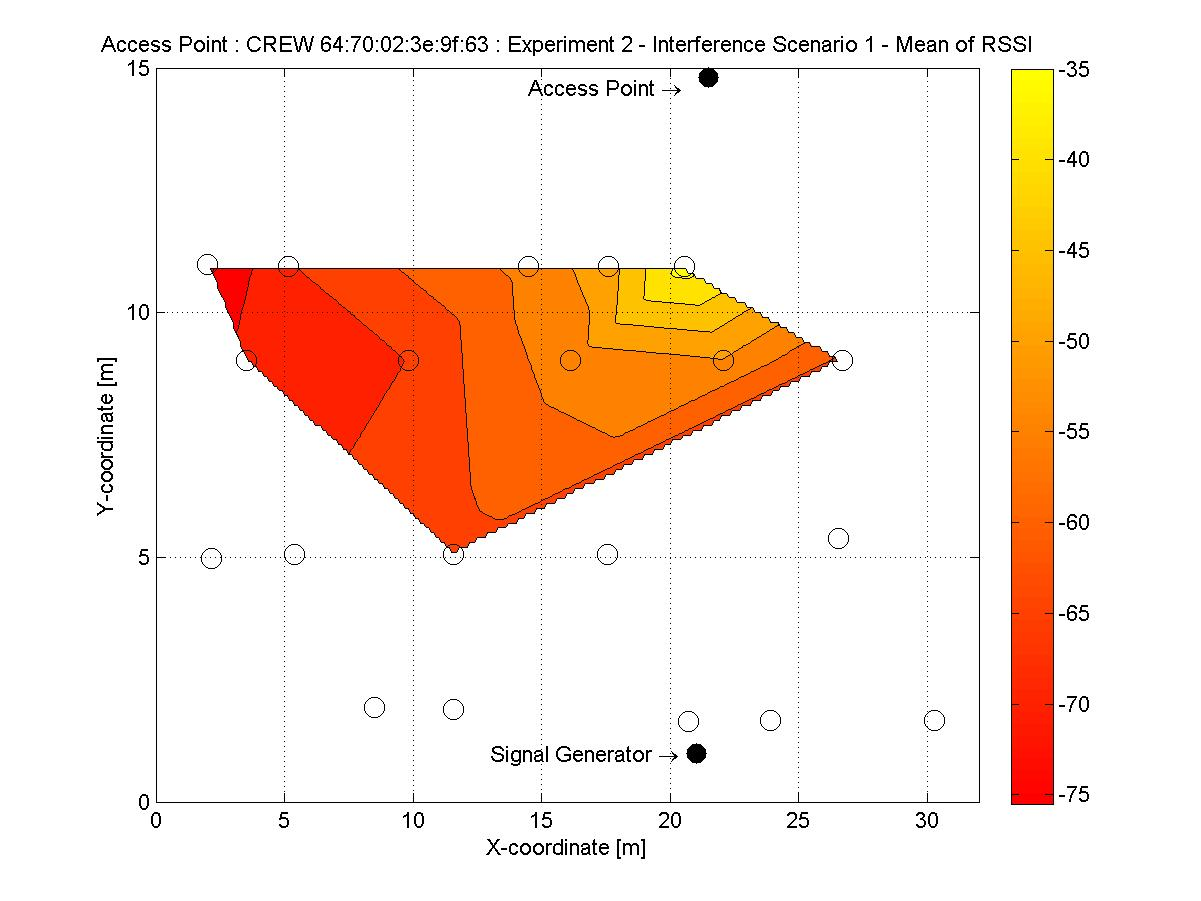
\includegraphics[width=13cm]{../../Source/plot/CREW_63/63_Sig_Ex_2_Mean.jpg} \\
	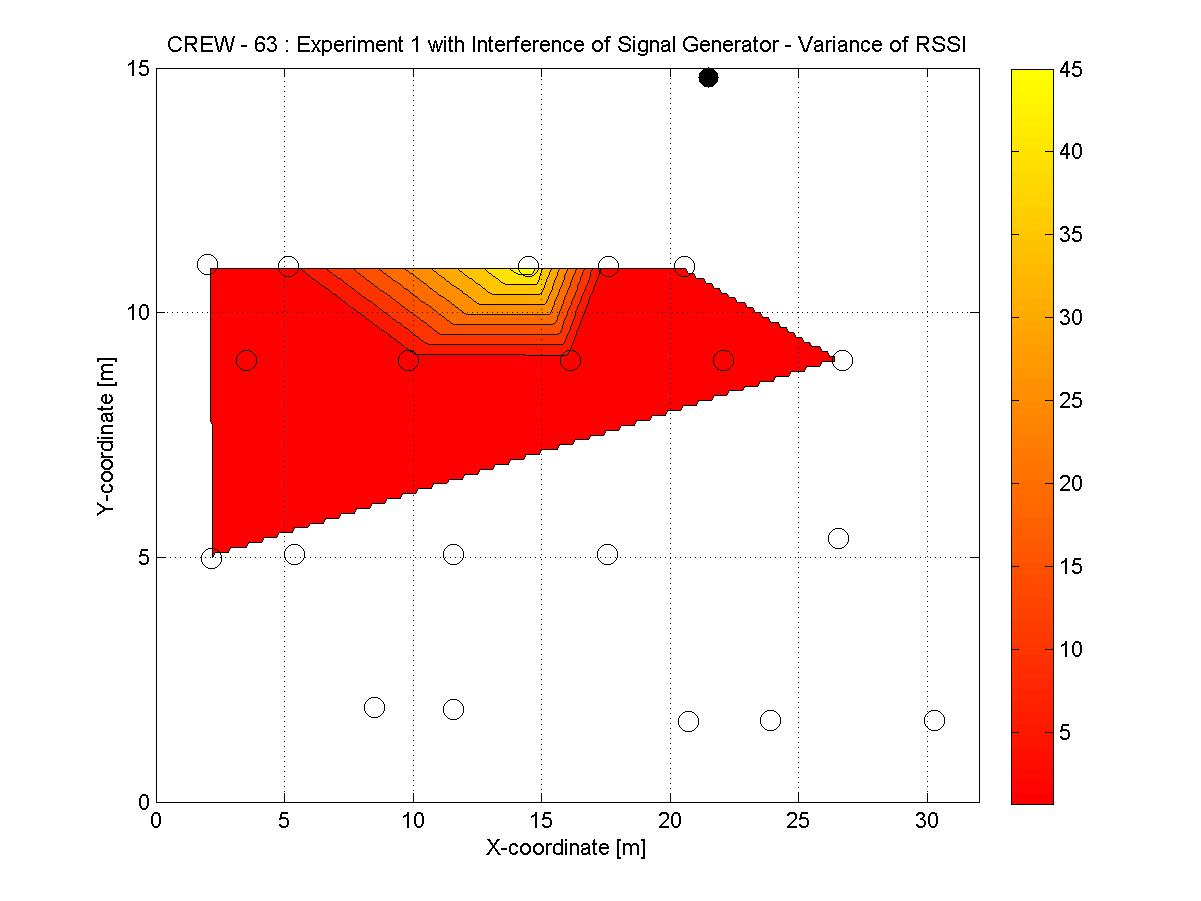
\includegraphics[width=13cm]{../../Source/plot/CREW_63/63_Sig_Ex_1_Variance.jpg} \\
	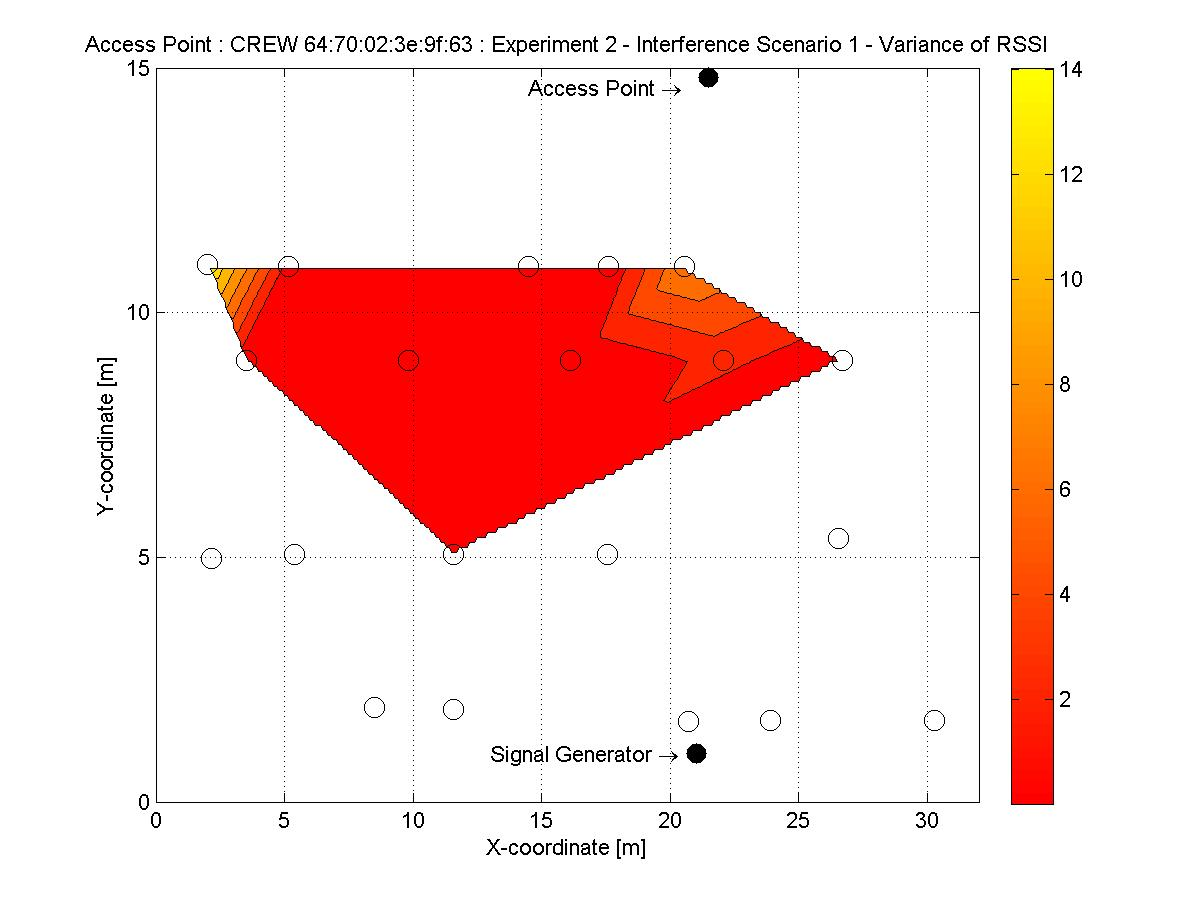
\includegraphics[width=13cm]{../../Source/plot/CREW_63/63_Sig_Ex_2_Variance.jpg} \\
\end{longtable}

\subsection{Interference Scenario 2} 
Following plots show mean and variance of RSSI values from the access point (CREW 64:70:02:3e:9f:63). Mean and Variance are plotted spatially with color map to show the significance. As described in the section \ref{scene:int:2}, these experiments were conducted in a scenario where interference is caused by Wifi data traffic between a server and email client, data client and video client.
\begin{longtable}
	{lr} 
	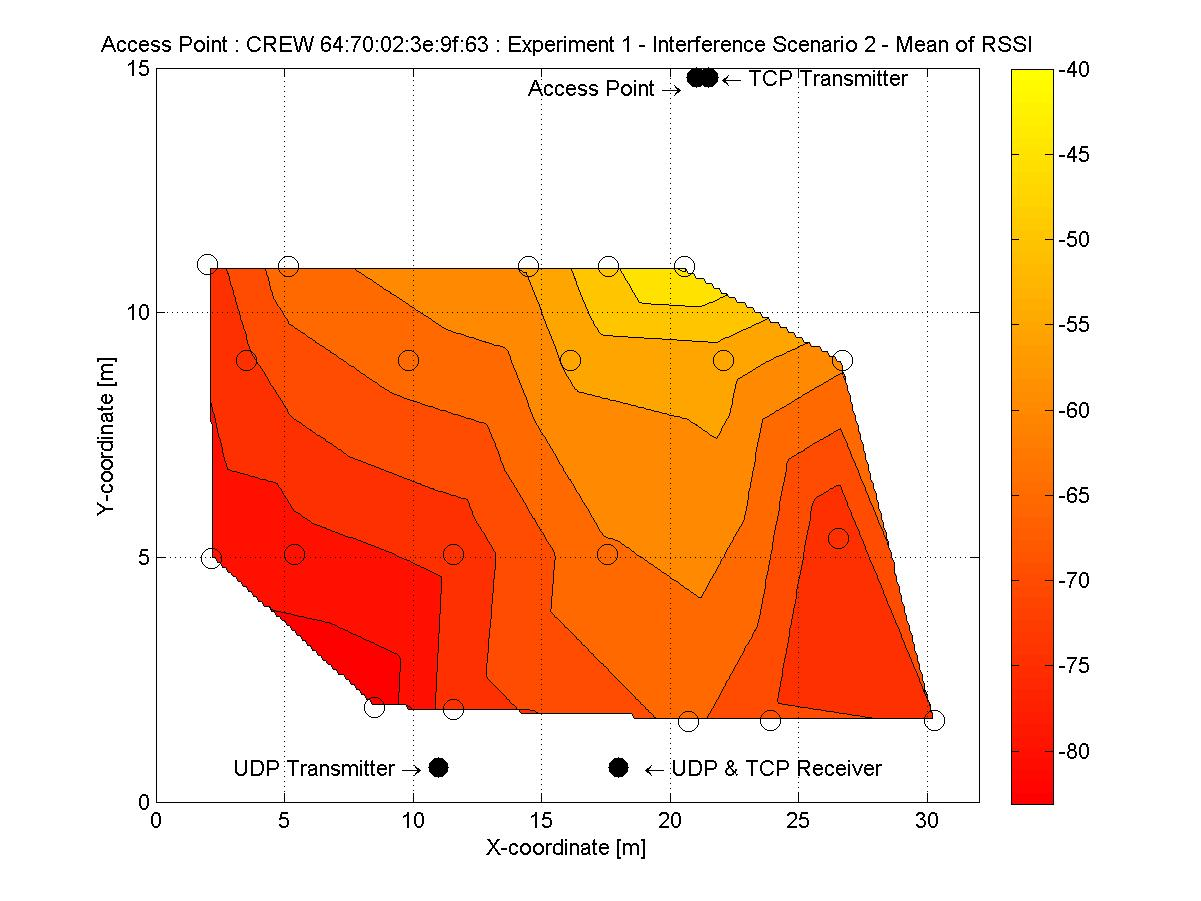
\includegraphics[width=13cm]{../../Source/plot/CREW_63/63_Wifi_Ex_1_Mean.jpg} \\
	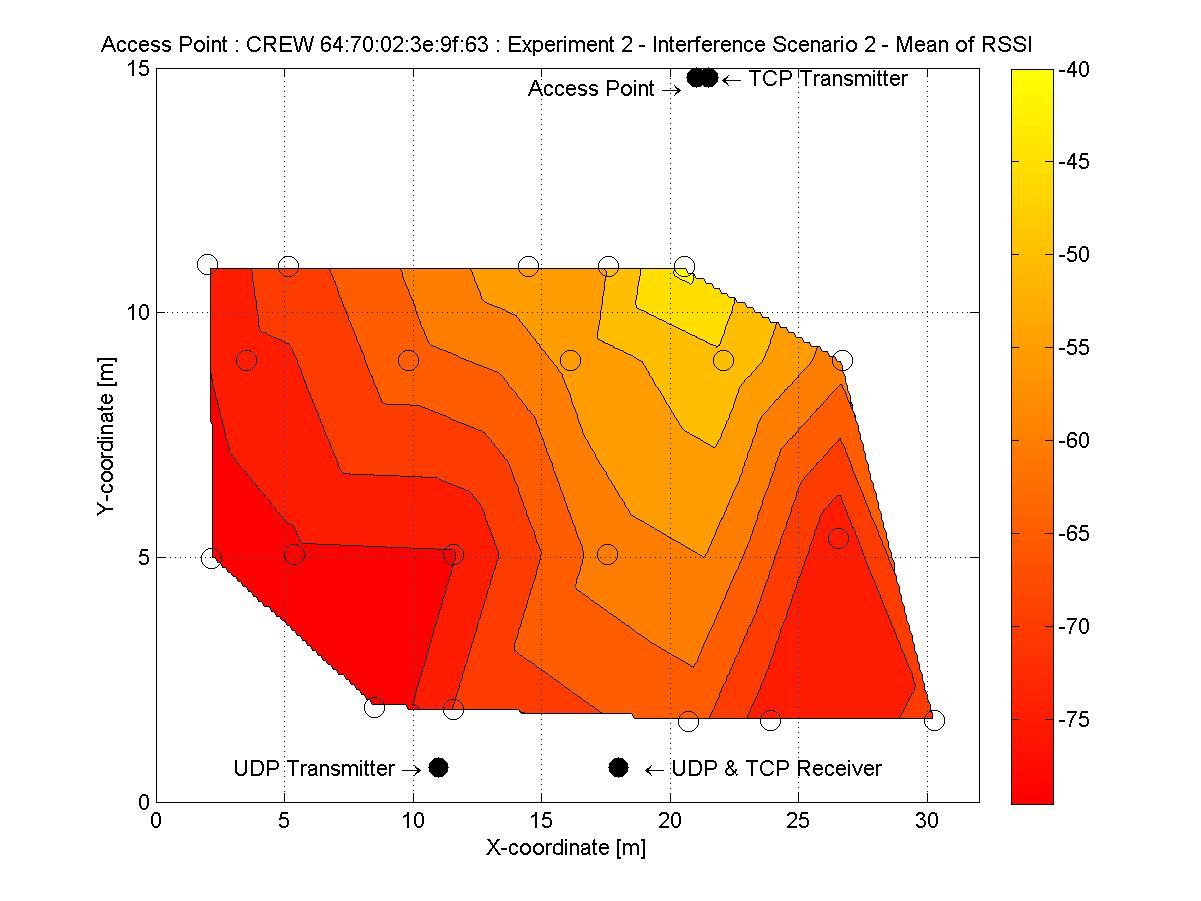
\includegraphics[width=13cm]{../../Source/plot/CREW_63/63_Wifi_Ex_2_Mean.jpg} \\
	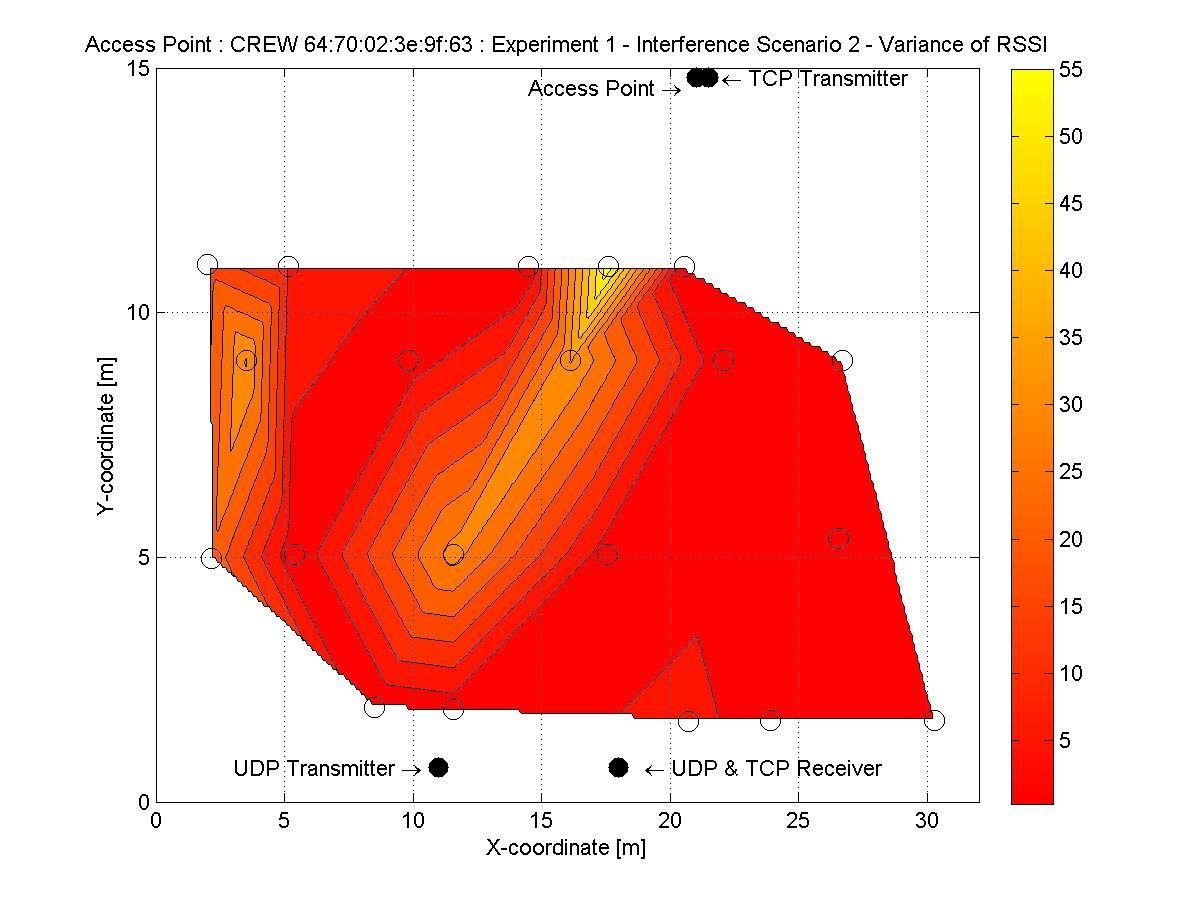
\includegraphics[width=13cm]{../../Source/plot/CREW_63/63_Wifi_Ex_1_Variance.jpg} \\
	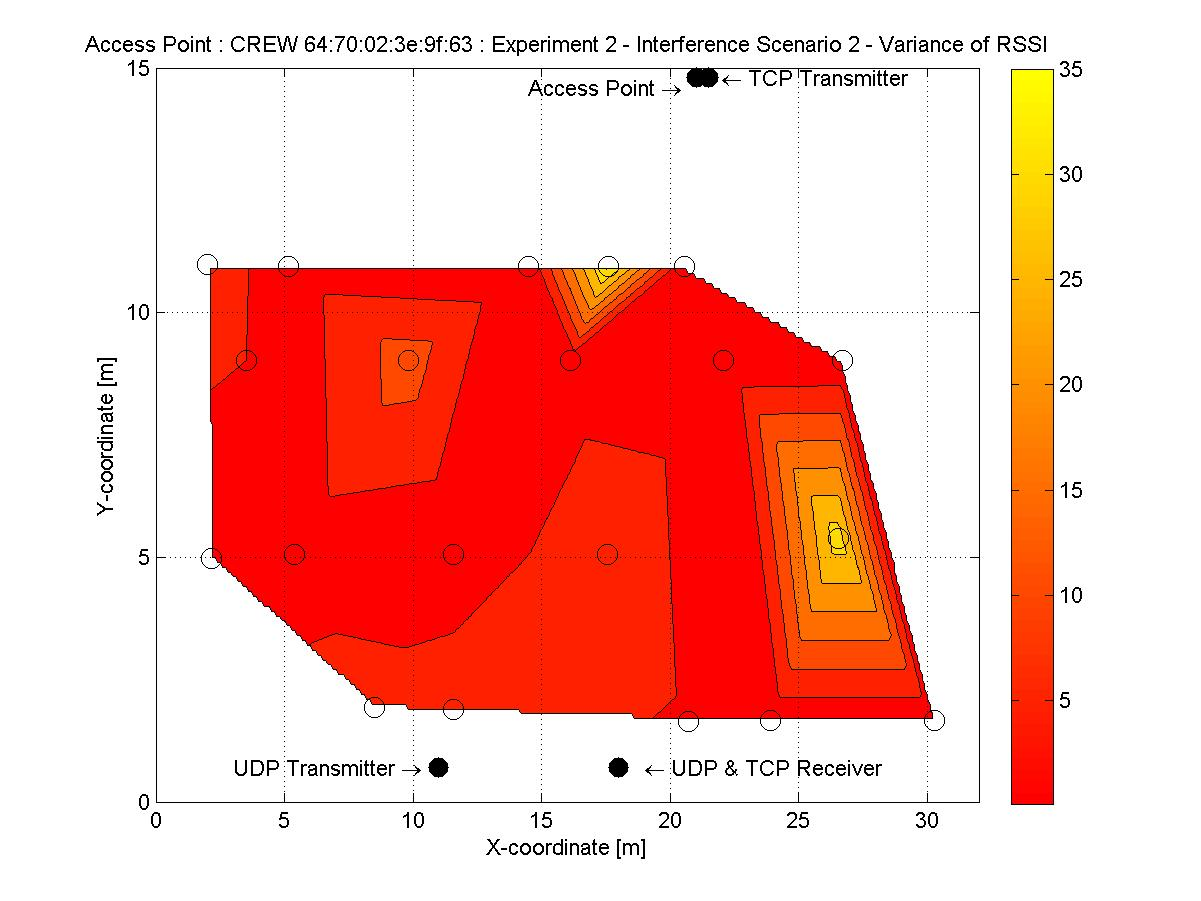
\includegraphics[width=13cm]{../../Source/plot/CREW_63/63_Wifi_Ex_2_Variance.jpg} \\
\end{longtable}

\subsection{Group Variances} 
Following plots show group variances of RSSI values from the access point (CREW 64:70:02:3e:9f:63) of experiments with reference scenario, interference scenario 1 and interference scenario 2. As described in the section \ref{sec:repeat}, Group variances are calculated.  
\begin{longtable}
	{lr} 
	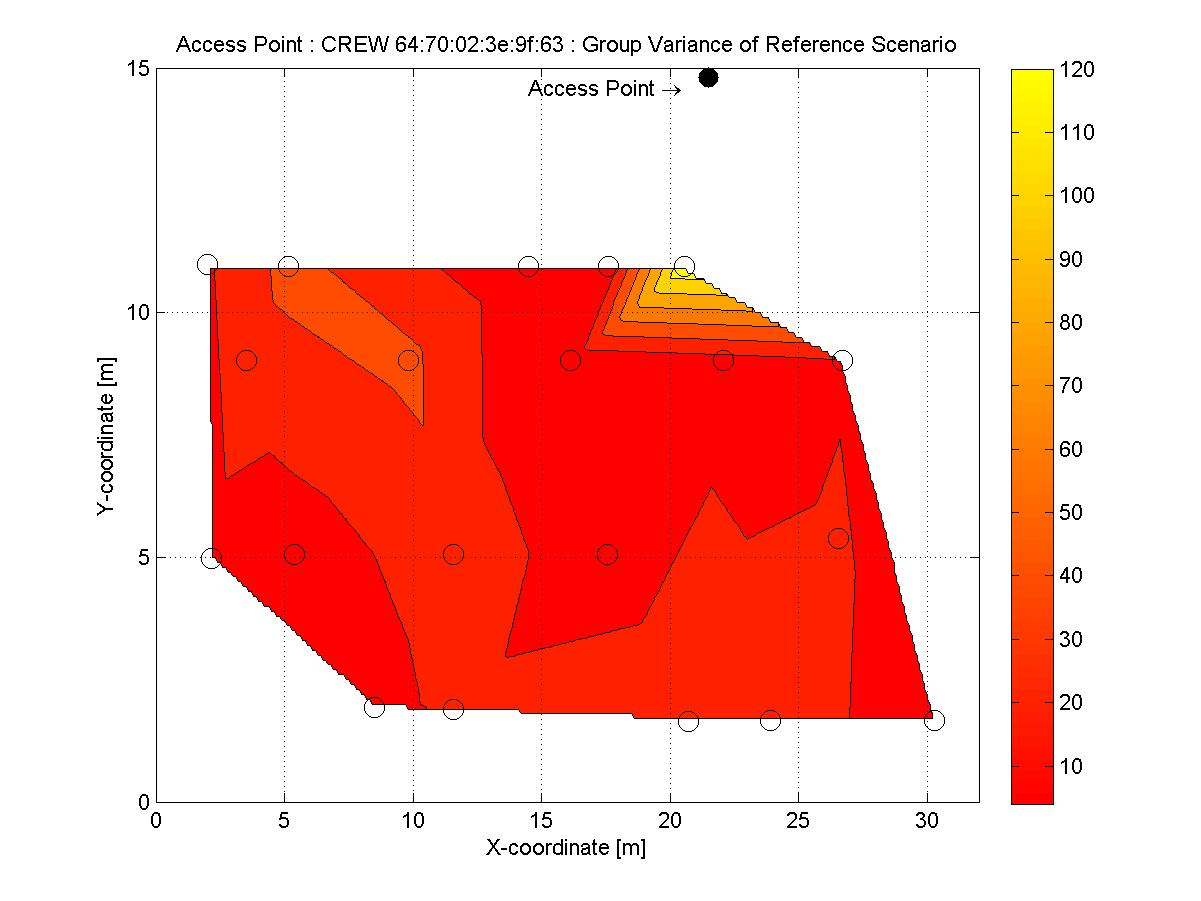
\includegraphics[width=13cm]{../../Source/plot/CREW_63/63_Ref_Group_Variance.jpg} \\
	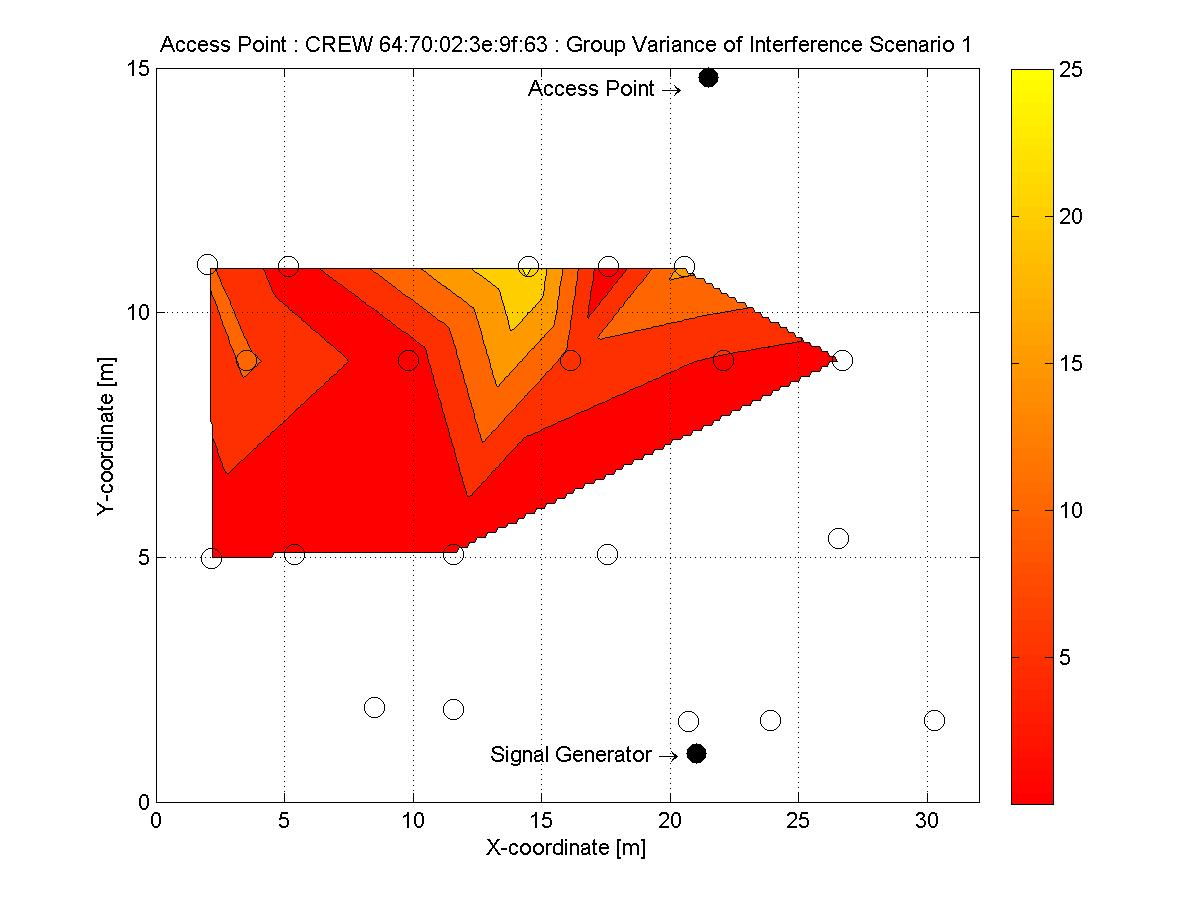
\includegraphics[width=13cm]{../../Source/plot/CREW_63/63_Sig_Group_Variance.jpg} \\
	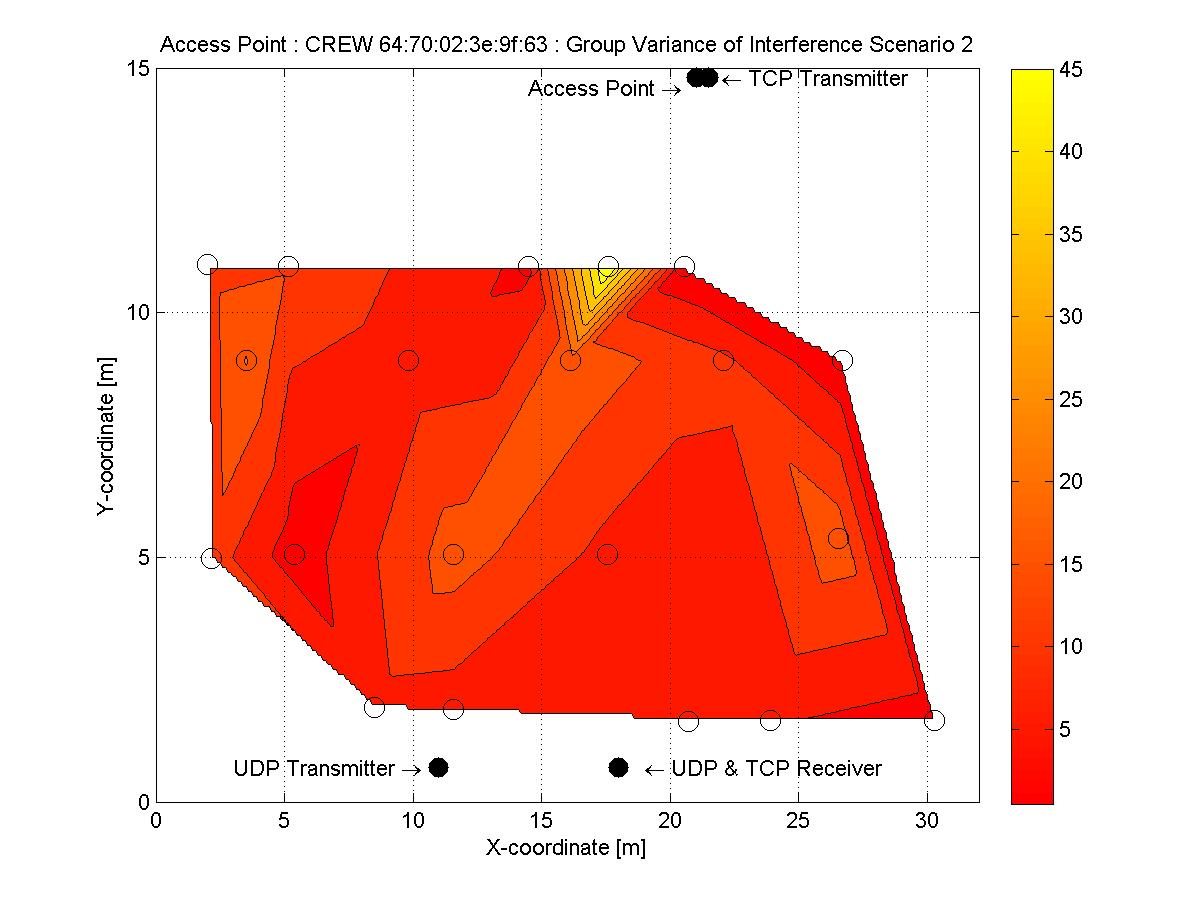
\includegraphics[width=13cm]{../../Source/plot/CREW_63/63_Wifi_Group_Variance.jpg} \\
\end{longtable}

\section{Access Point : CREW 64:70:02:3e:aa:11} 
The details of the access point are given below.
\begin{itemize}
	\item SSID : CREW 
	\item BSSID : 64:70:02:3e:aa:11 
	\item Location : X-axis - 31.0m, Y-axis - 0.7m 
	\item Frequency : 2.4 GHz 
\end{itemize}
\subsection{Reference Scenario} 
Following plots show mean and variance of RSSI values from the access point (CREW 64:70:02:3e:aa:11). Mean and Variance are plotted spatially with color map to show the significance. As described in the section \ref{scene:ref}, these experiments were conducted in a scenario where no artificial interference is generated and the presence of uncontrolled interference is minimized.
\begin{longtable}
	{lr} 
	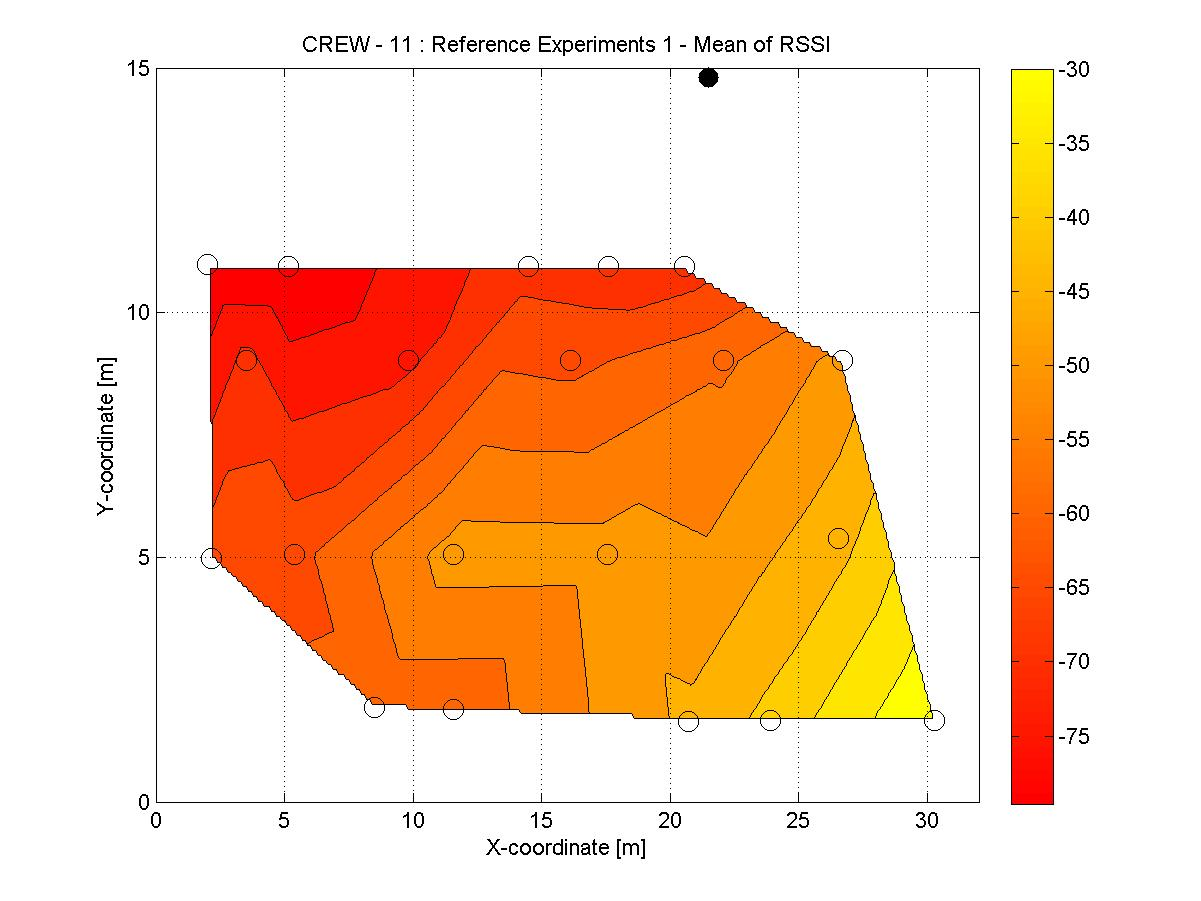
\includegraphics[width=13cm]{../../Source/plot/CREW_11/11_Ref_Ex_1_Mean.jpg} \\
	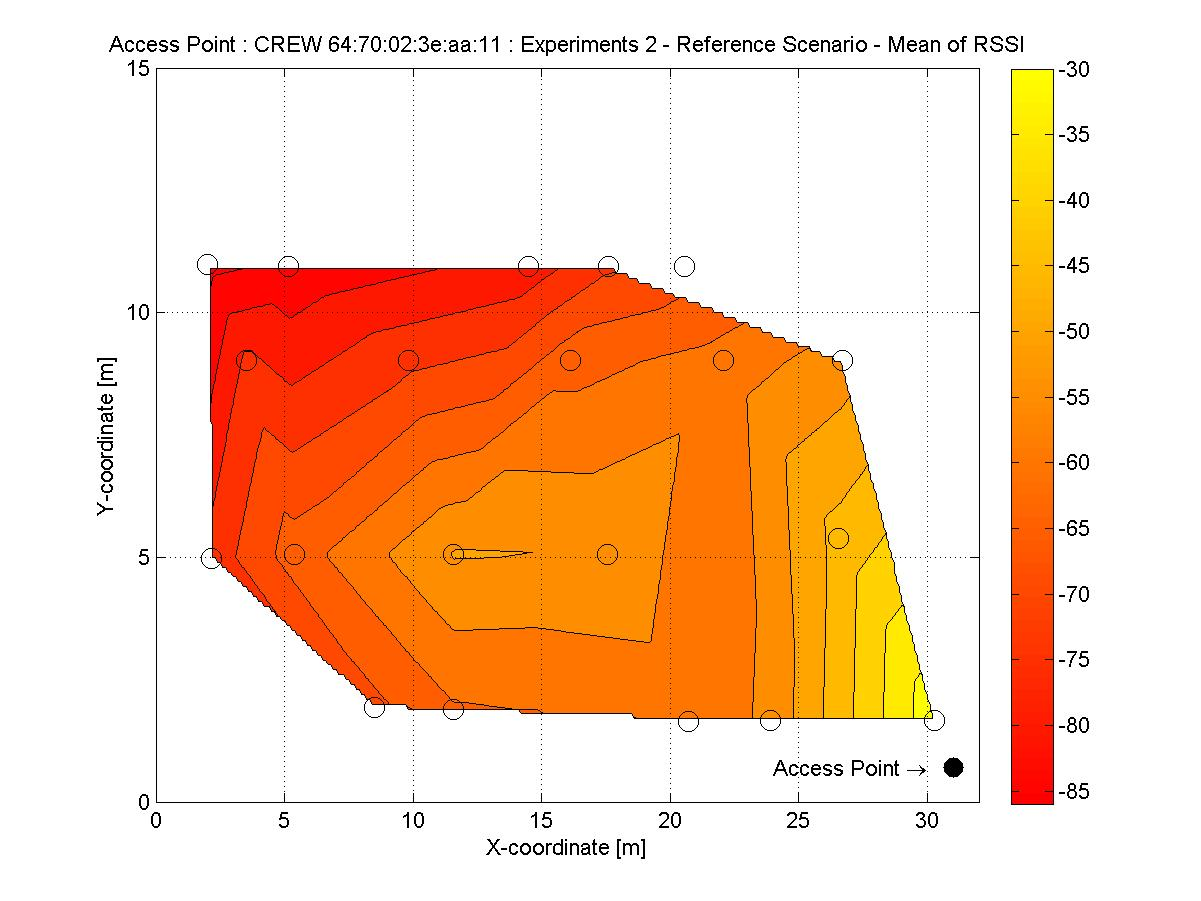
\includegraphics[width=13cm]{../../Source/plot/CREW_11/11_Ref_Ex_2_Mean.jpg} \\
	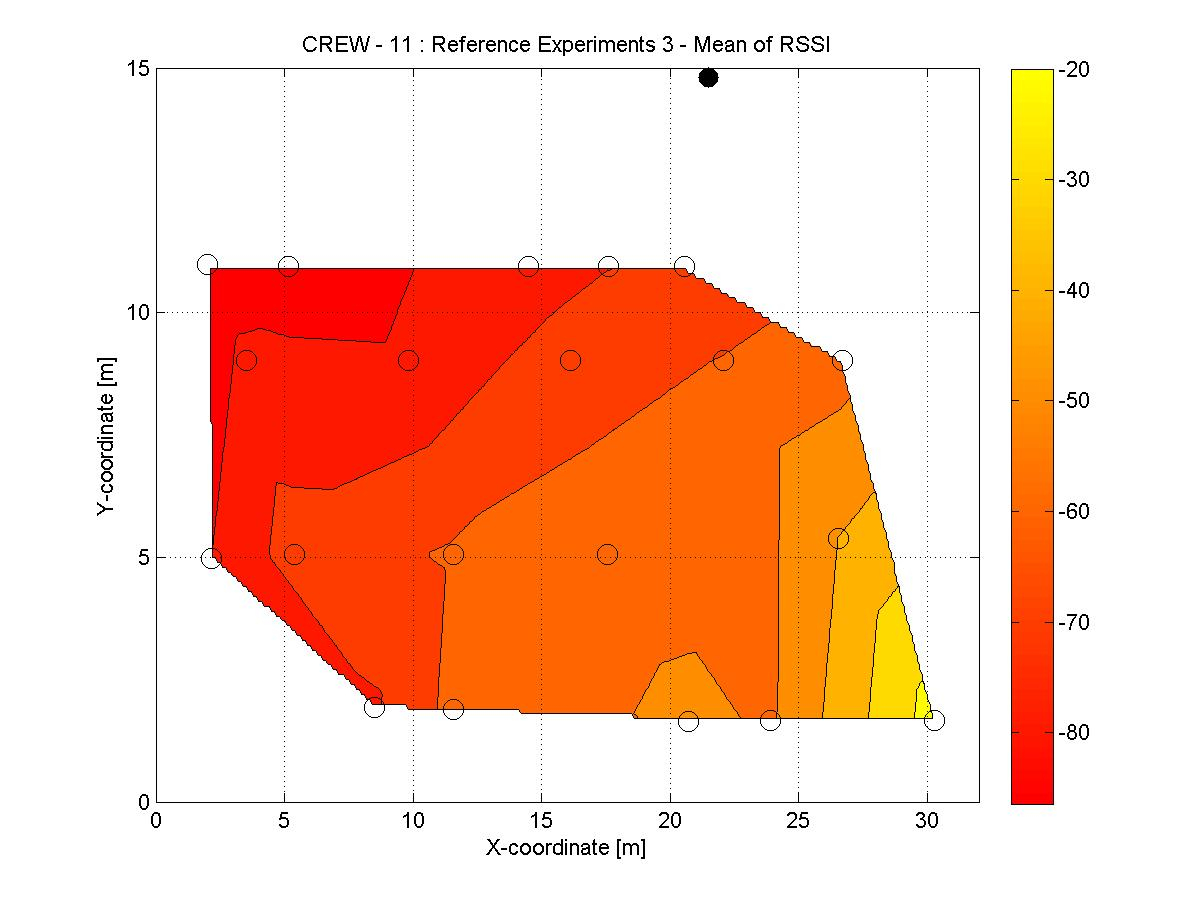
\includegraphics[width=13cm]{../../Source/plot/CREW_11/11_Ref_Ex_3_Mean.jpg} \\
	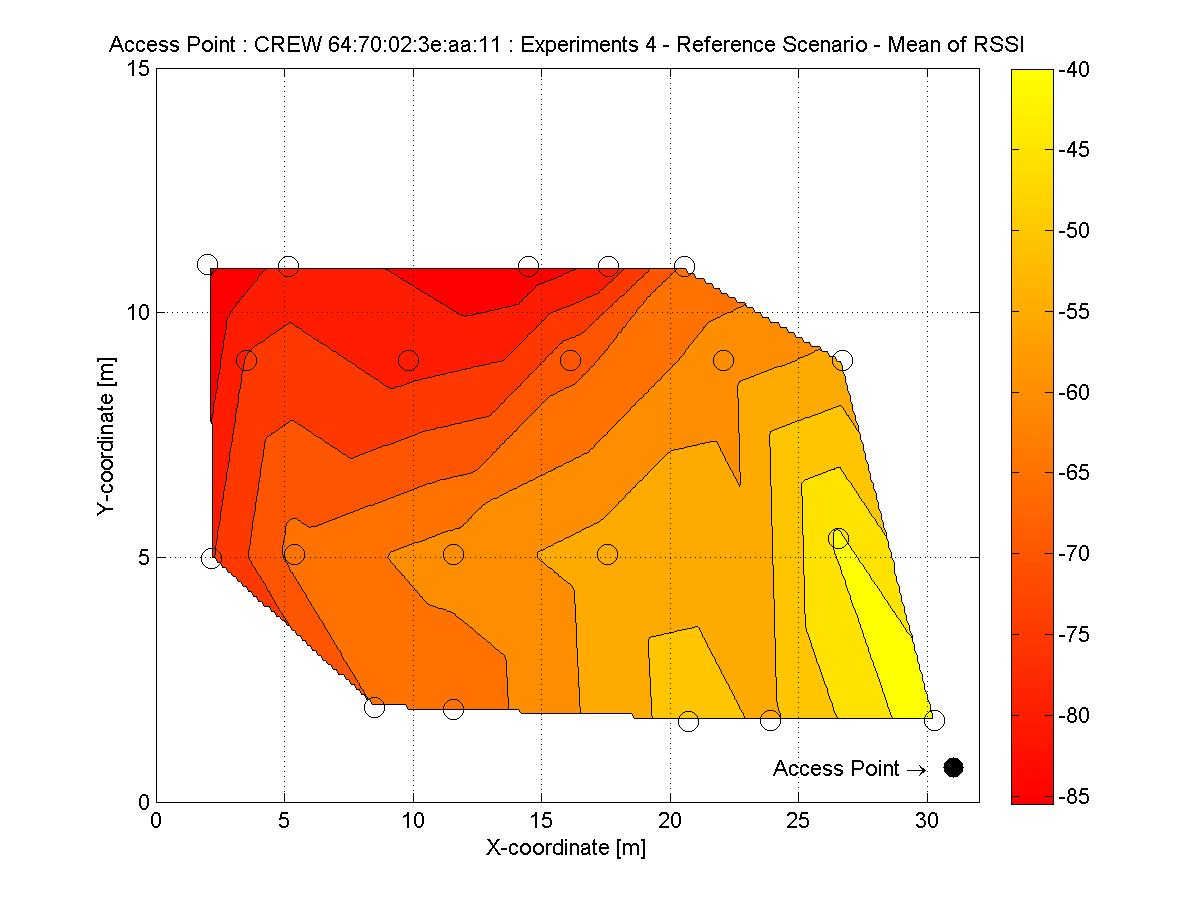
\includegraphics[width=13cm]{../../Source/plot/CREW_11/11_Ref_Ex_4_Mean.jpg} \\
	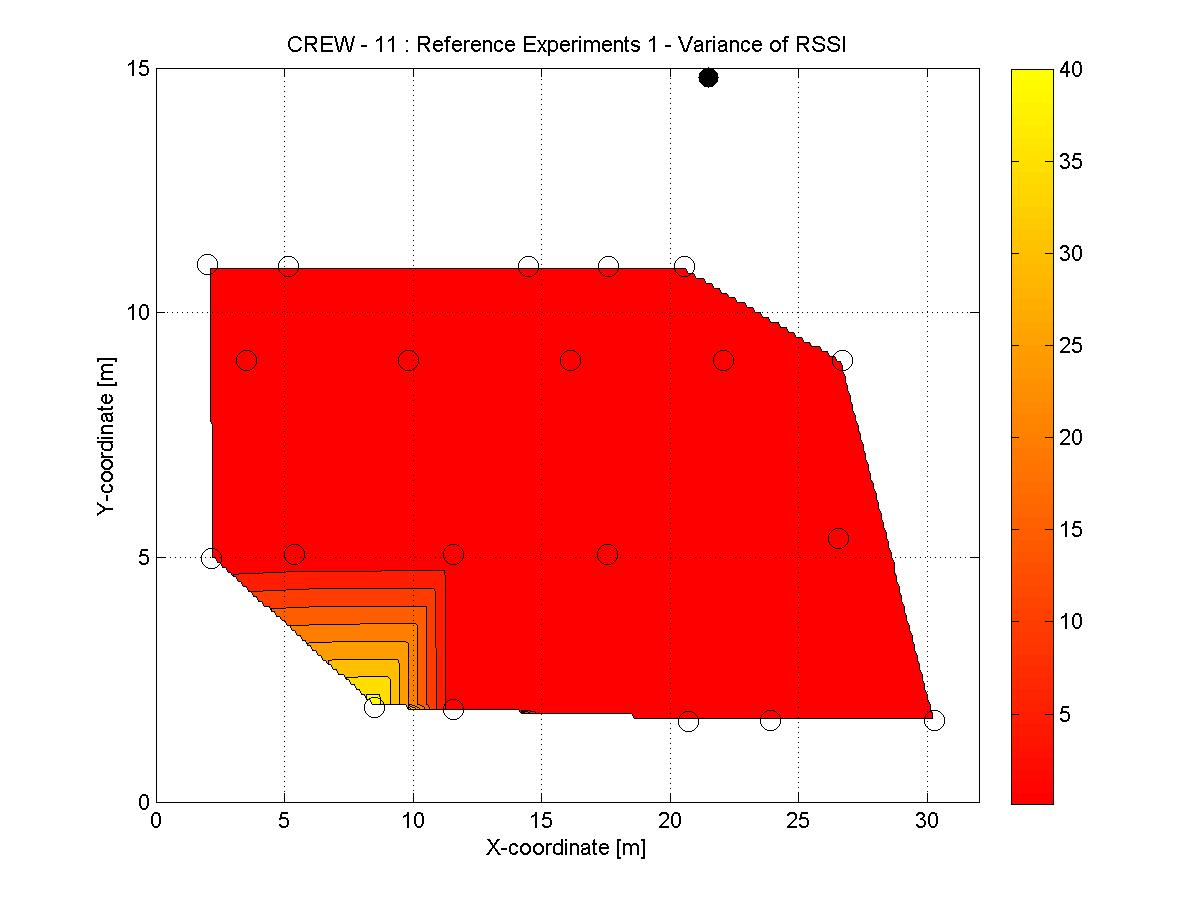
\includegraphics[width=13cm]{../../Source/plot/CREW_11/11_Ref_Ex_1_Variance.jpg} \\
	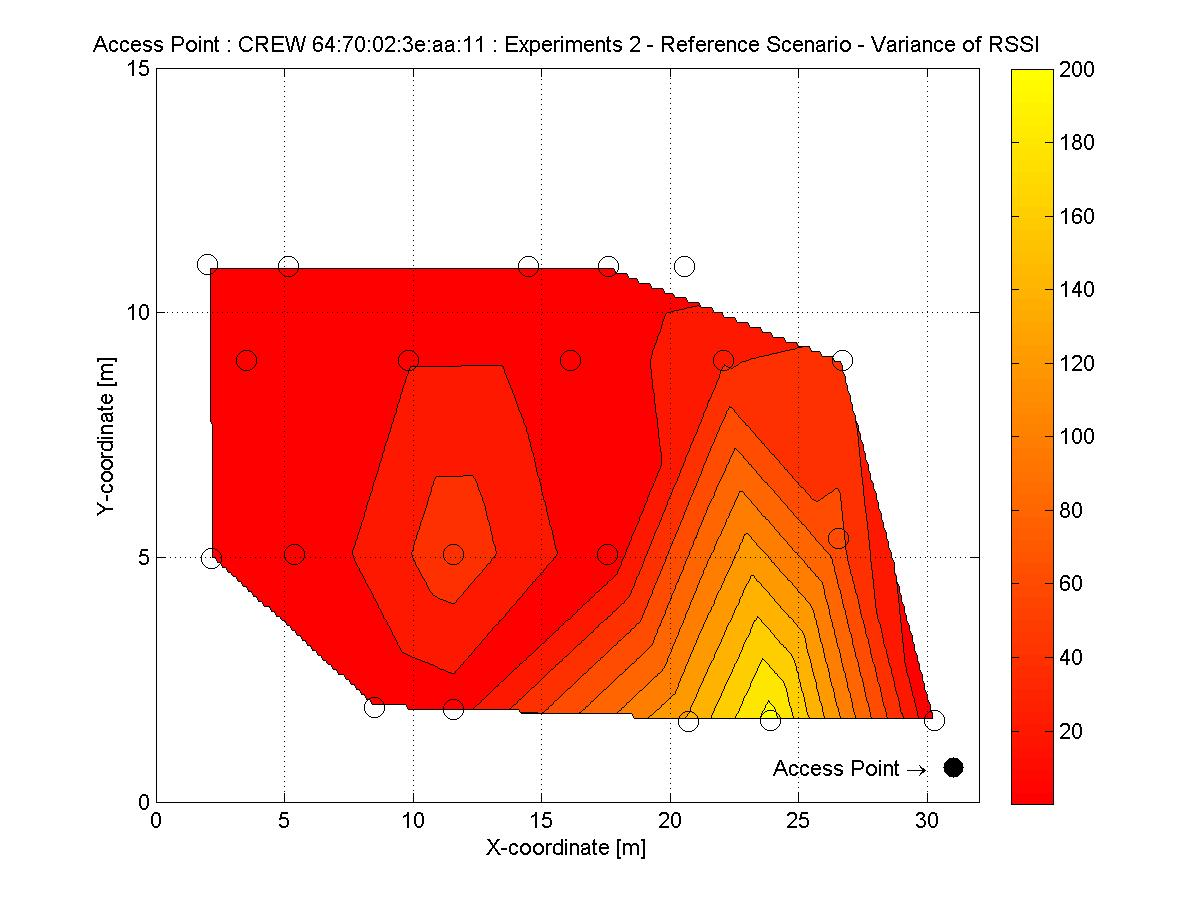
\includegraphics[width=13cm]{../../Source/plot/CREW_11/11_Ref_Ex_2_Variance.jpg} \\
	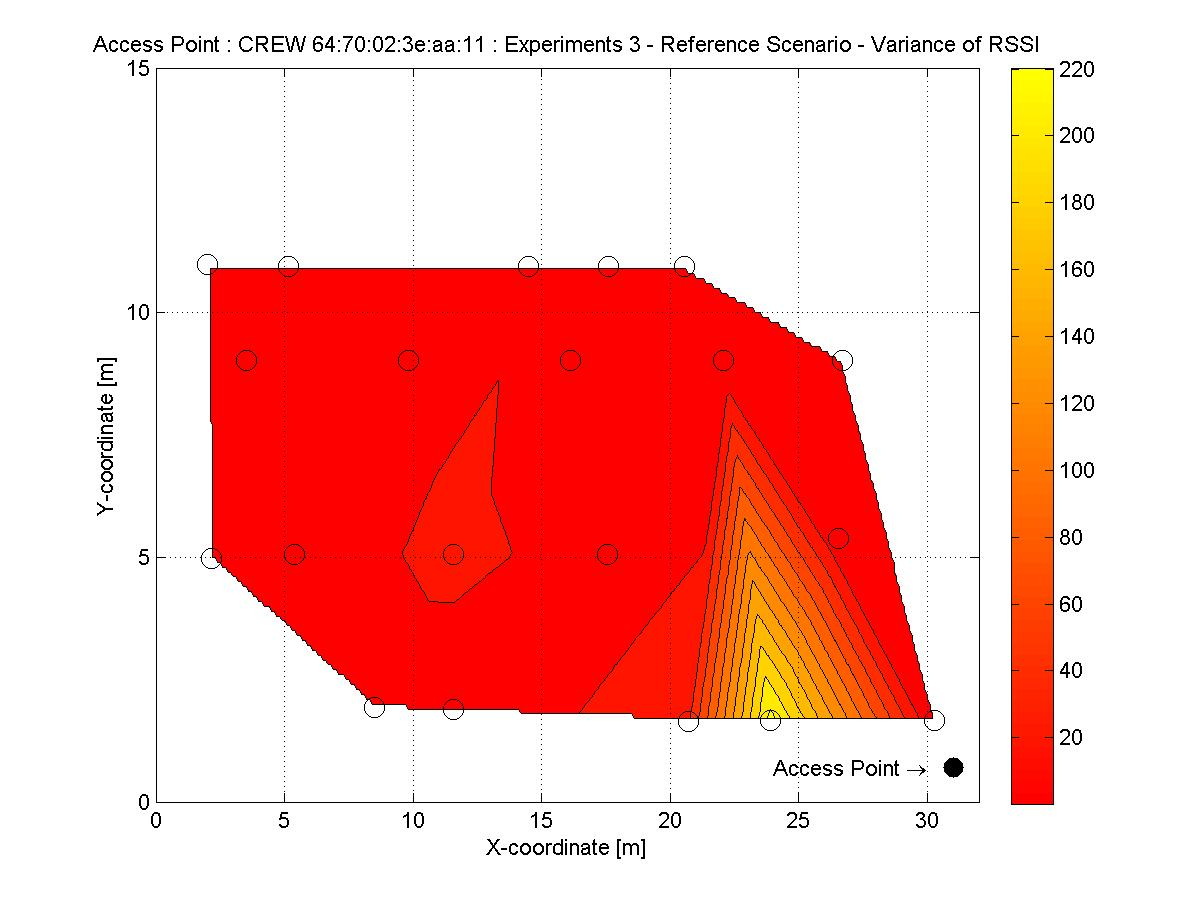
\includegraphics[width=13cm]{../../Source/plot/CREW_11/11_Ref_Ex_3_Variance.jpg} \\
	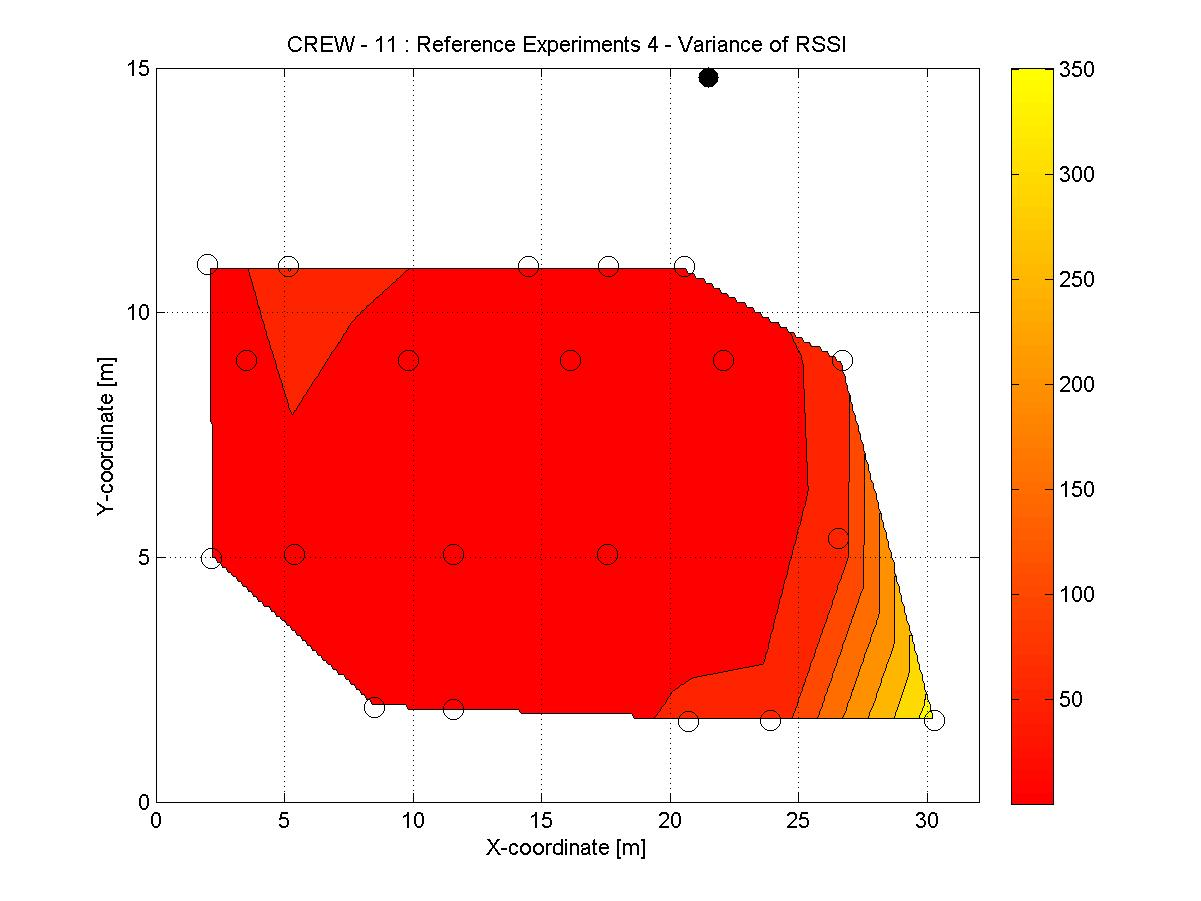
\includegraphics[width=13cm]{../../Source/plot/CREW_11/11_Ref_Ex_4_Variance.jpg} 
\end{longtable}

\subsection{Interference Scenario 1} 
Following plots show mean and variance of RSSI values from the access point (CREW 64:70:02:3e:aa:11). Mean and Variance are plotted spatially with color map to show the significance. As described in the section \ref{scene:int:1}, these experiments were conducted in a scenario where IEEE 802.11 channel was jammed with the maximum transmission power using signal generators.
\begin{longtable}
	{lr} 
	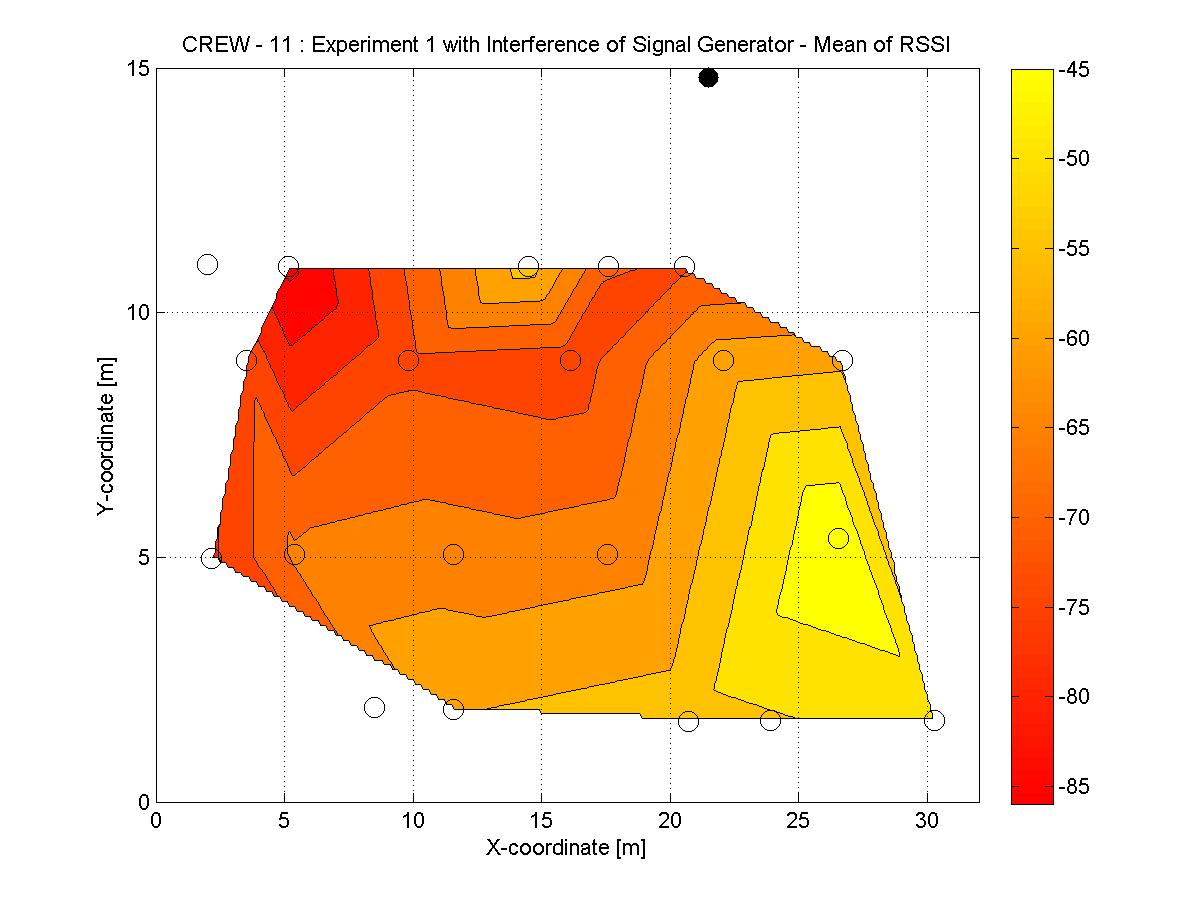
\includegraphics[width=13cm]{../../Source/plot/CREW_11/11_Sig_Ex_1_Mean.jpg} \\
	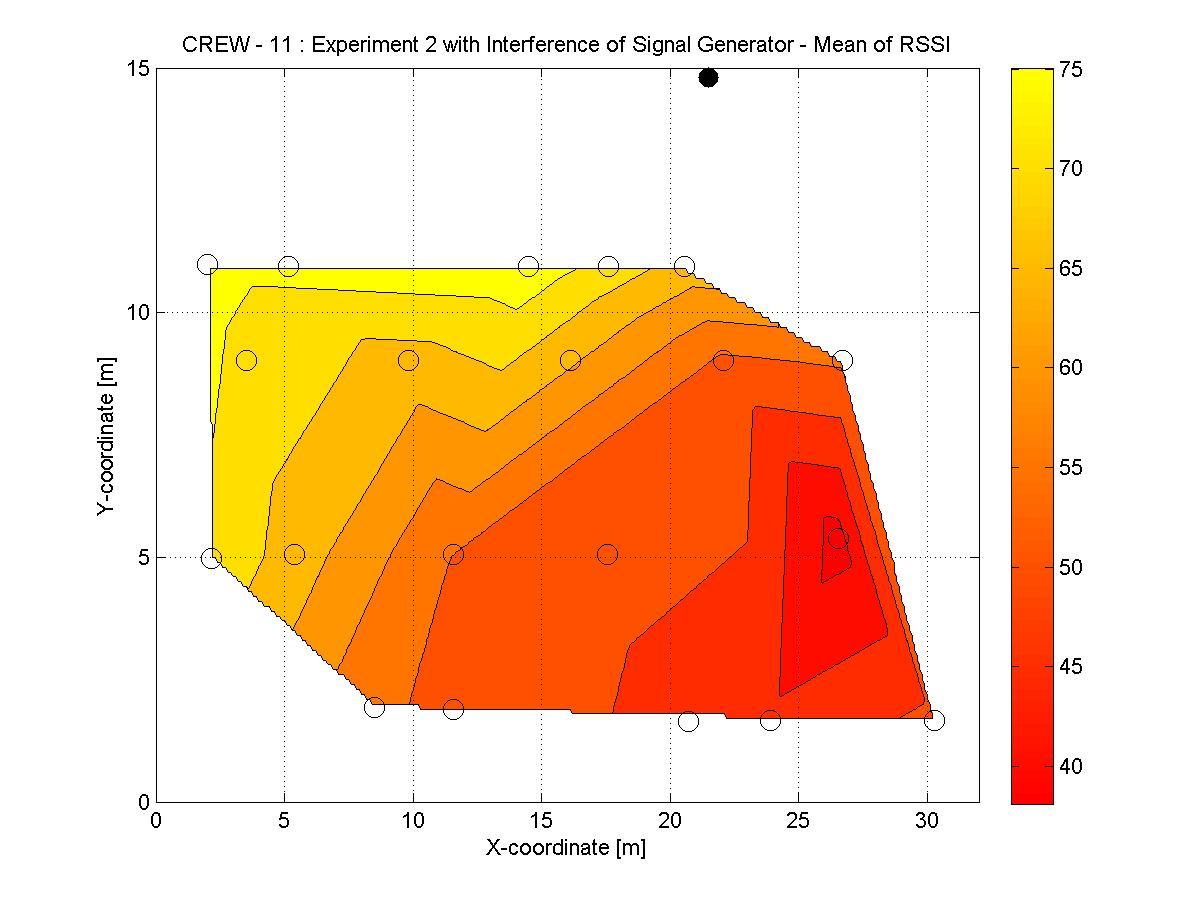
\includegraphics[width=13cm]{../../Source/plot/CREW_11/11_Sig_Ex_2_Mean.jpg} \\
	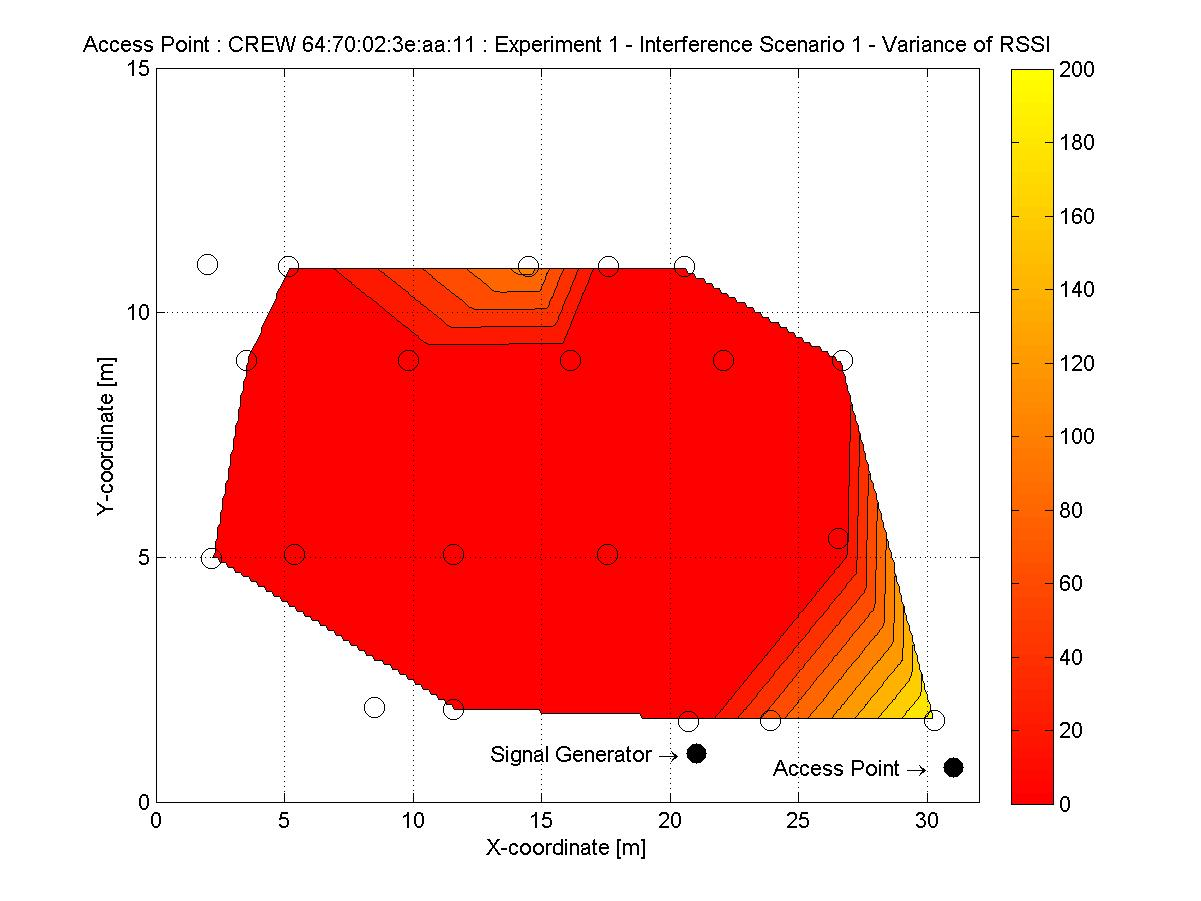
\includegraphics[width=13cm]{../../Source/plot/CREW_11/11_Sig_Ex_1_Variance.jpg} \\
	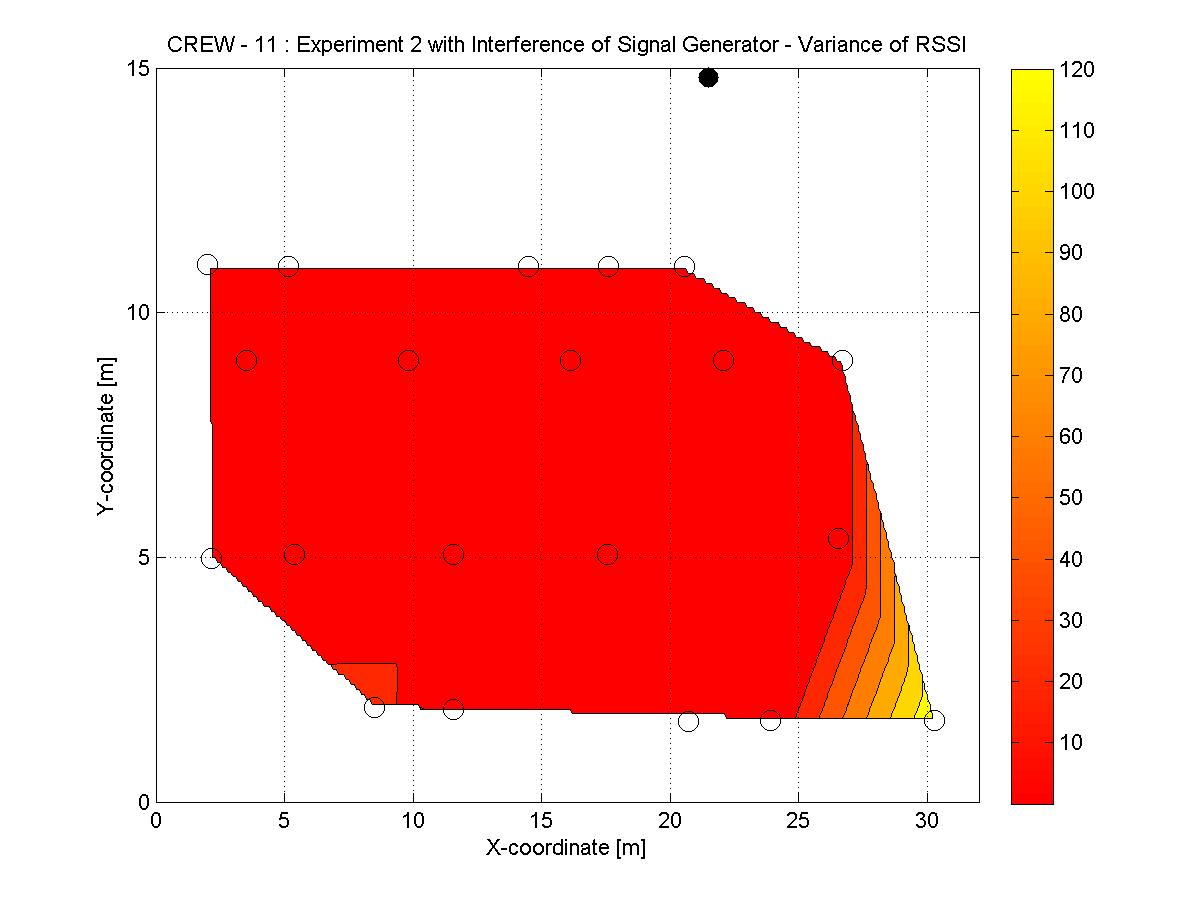
\includegraphics[width=13cm]{../../Source/plot/CREW_11/11_Sig_Ex_2_Variance.jpg} \\
\end{longtable}

\subsection{Interference Scenario 2} 
Following plots show mean and variance of RSSI values from the access point (CREW 64:70:02:3e:aa:11). Mean and Variance are plotted spatially with color map to show the significance. As described in the section \ref{scene:int:2}, these experiments were conducted in a scenario where interference is caused by Wifi data traffic between a server and email client, data client and video client.
\begin{longtable}
	{lr} 
	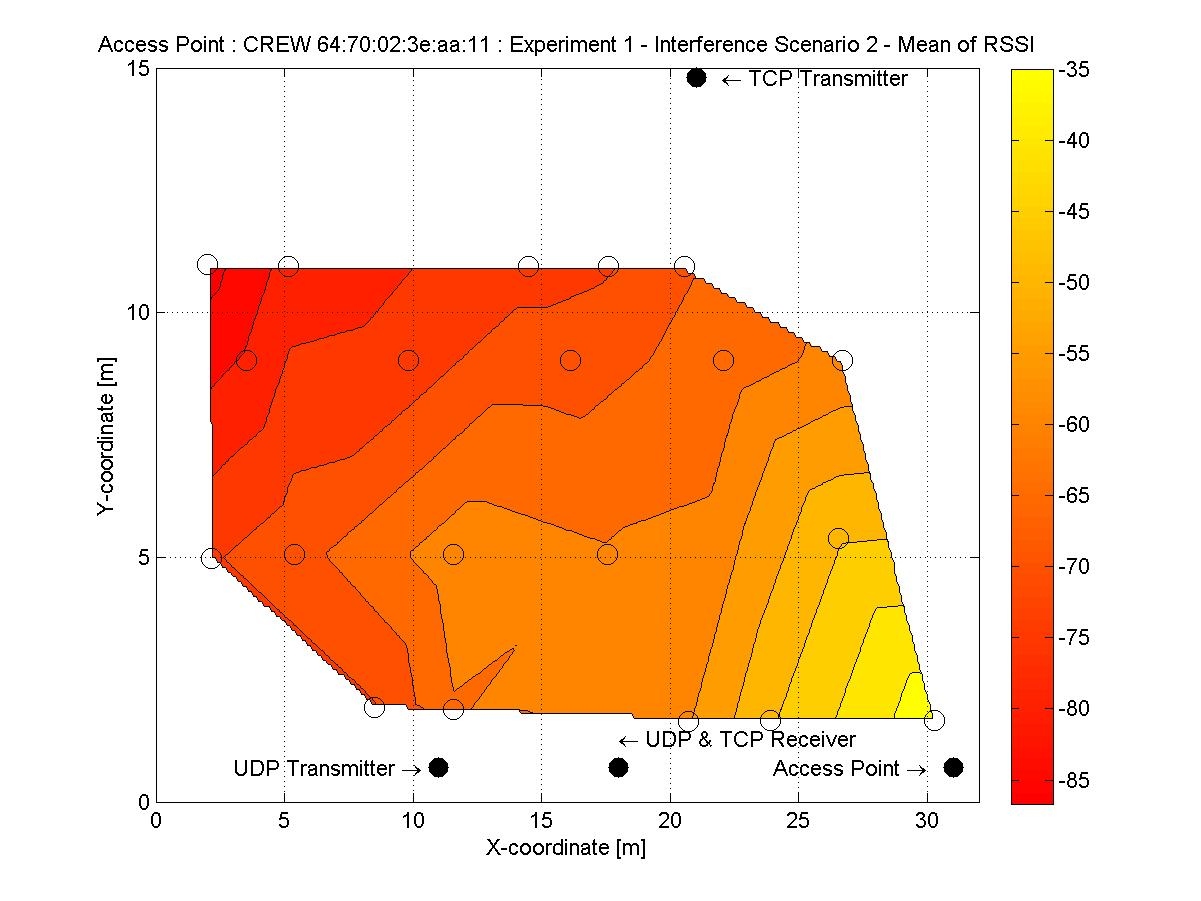
\includegraphics[width=13cm]{../../Source/plot/CREW_11/11_Wifi_Ex_1_Mean.jpg} \\
	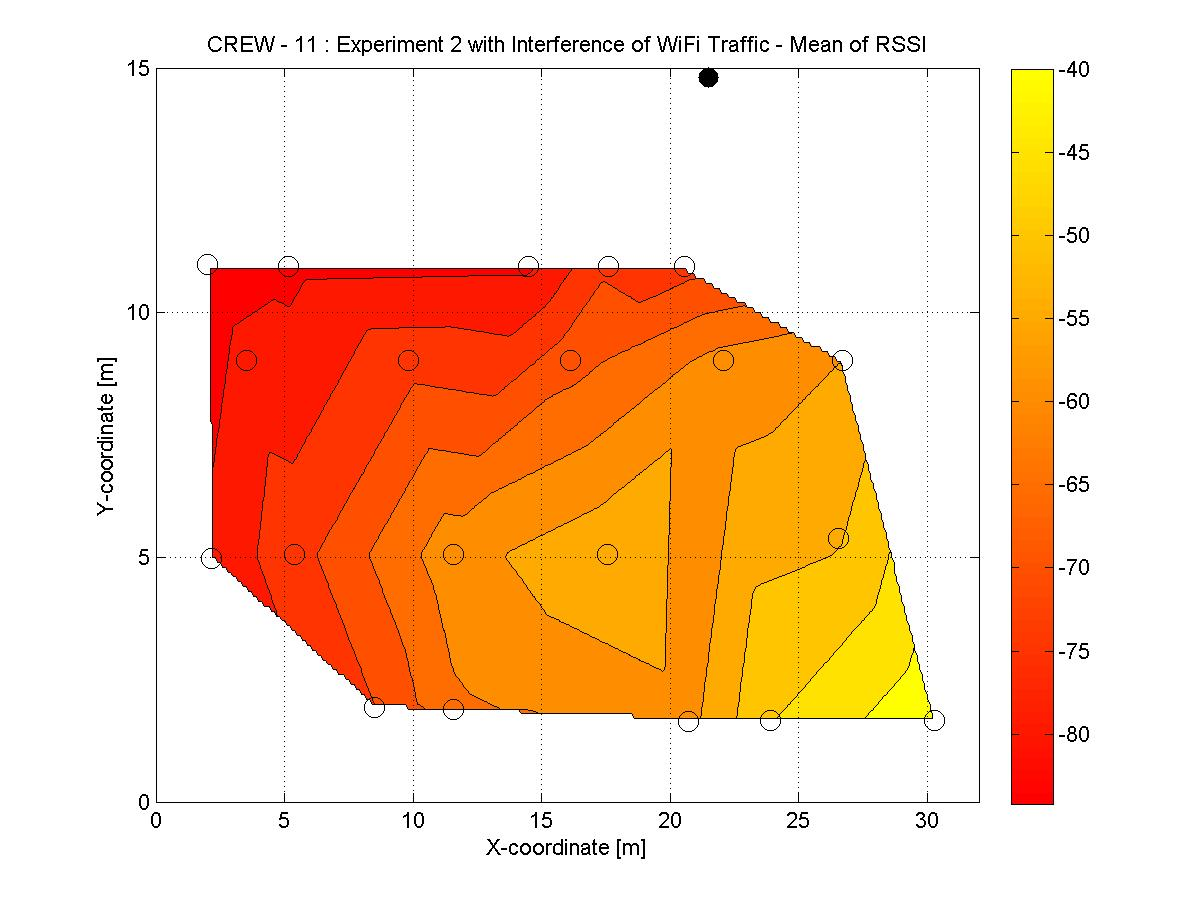
\includegraphics[width=13cm]{../../Source/plot/CREW_11/11_Wifi_Ex_2_Mean.jpg} \\
	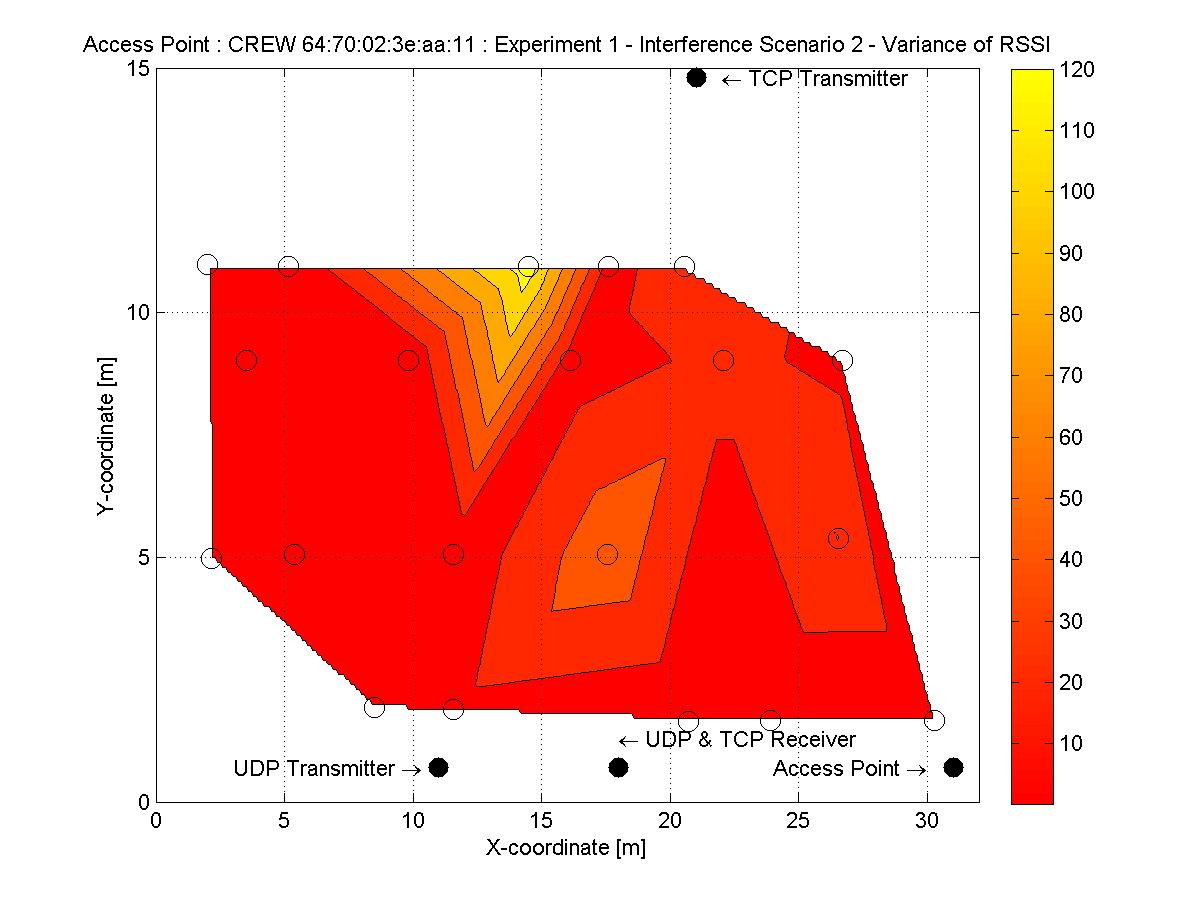
\includegraphics[width=13cm]{../../Source/plot/CREW_11/11_Wifi_Ex_1_Variance.jpg} \\
	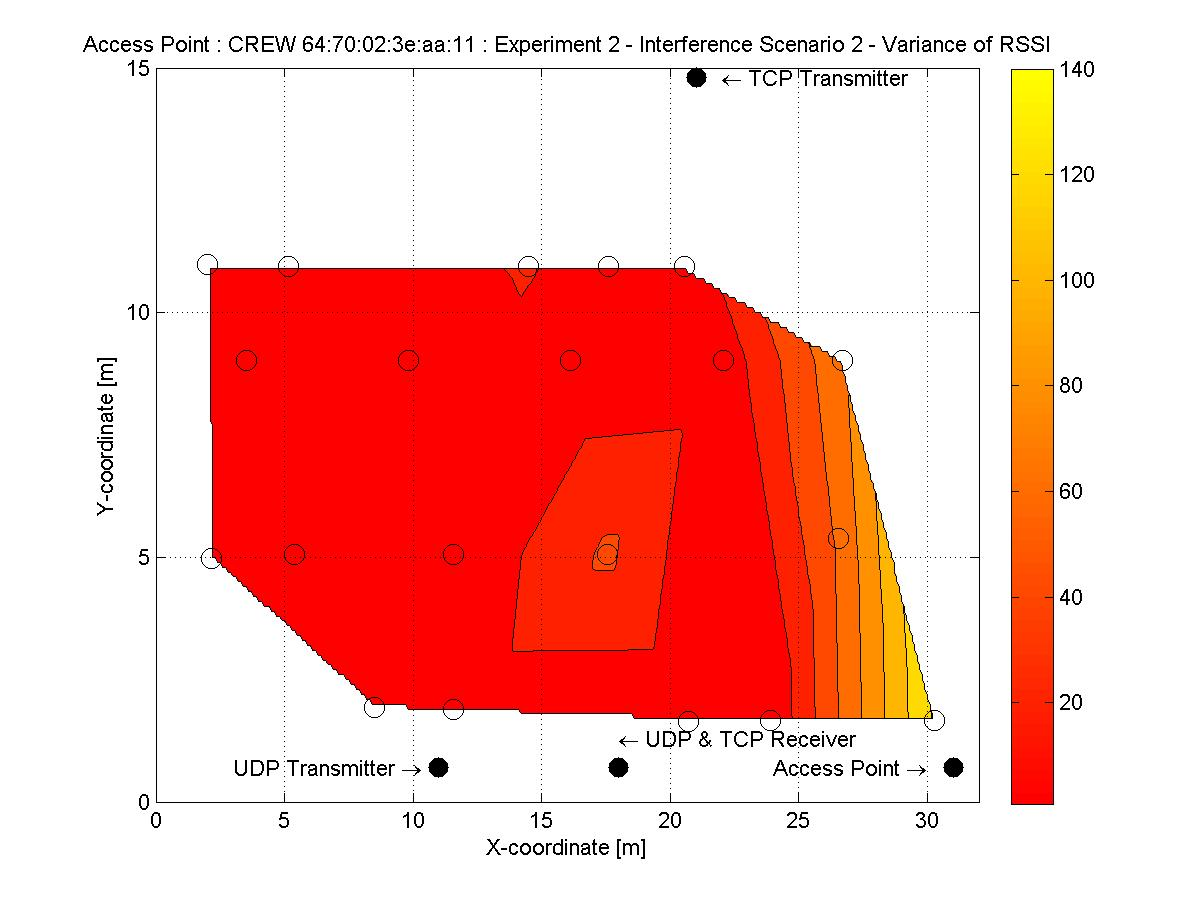
\includegraphics[width=13cm]{../../Source/plot/CREW_11/11_Wifi_Ex_2_Variance.jpg} \\
\end{longtable}

\subsection{Group Variances} 
Following plots show group variances of RSSI values from the access point (CREW 64:70:02:3e:aa:11) of experiments with reference scenario, interference scenario 1 and interference scenario 2. As described in the section \ref{sec:repeat}, Group variances are calculated.  
\begin{longtable}
	{lr} 
	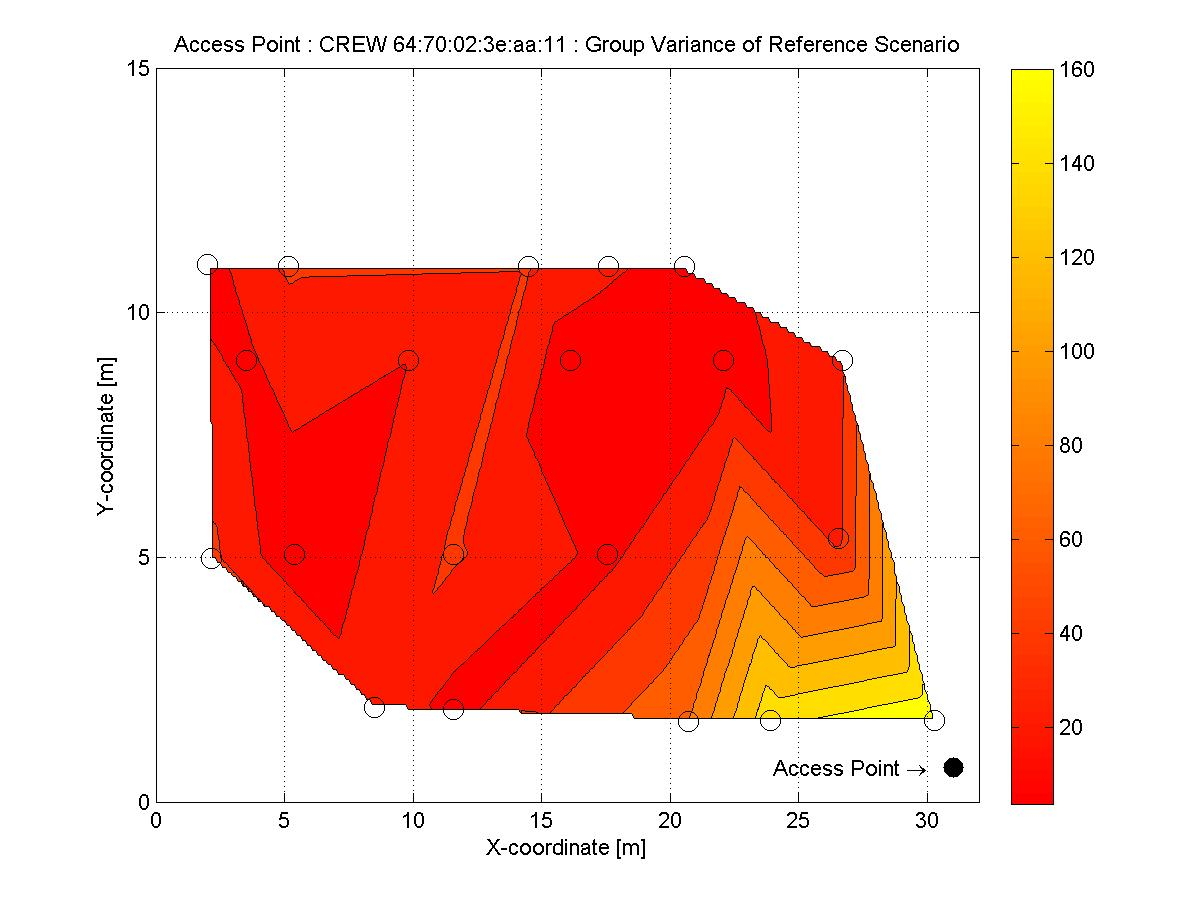
\includegraphics[width=13cm]{../../Source/plot/CREW_11/11_Ref_Group_Variance.jpg} \\
	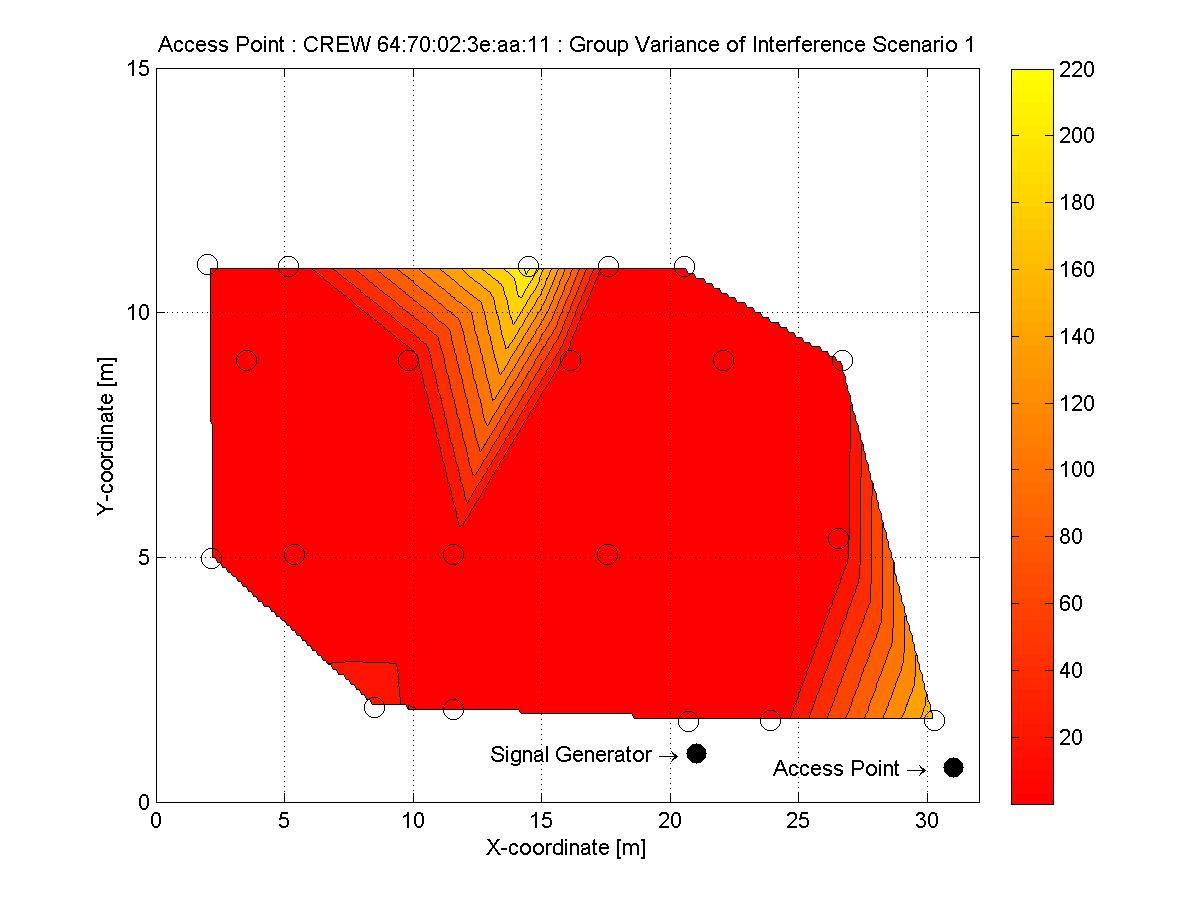
\includegraphics[width=13cm]{../../Source/plot/CREW_11/11_Sig_Group_Variance.jpg} \\
	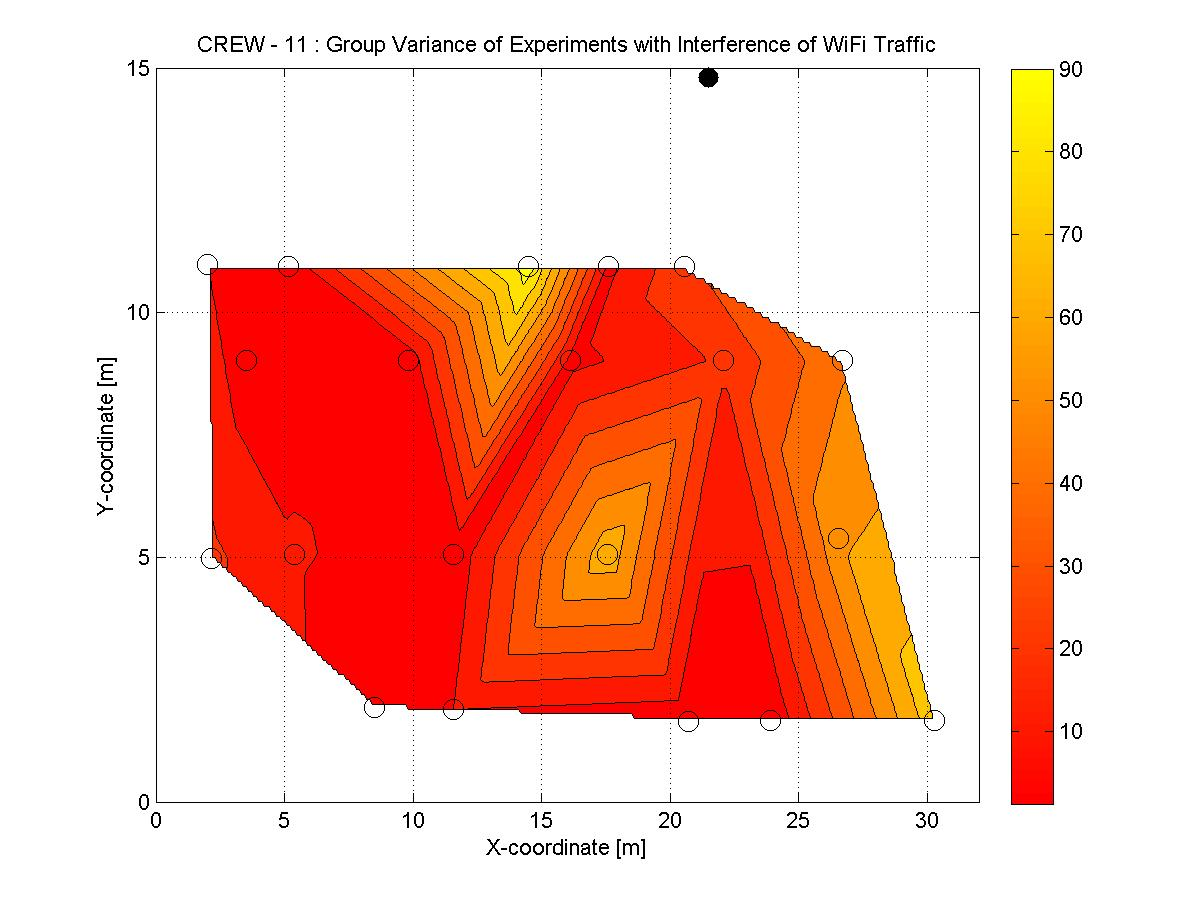
\includegraphics[width=13cm]{../../Source/plot/CREW_11/11_Wifi_Group_Variance.jpg} \\
\end{longtable}
\section{Access Point : CREW 64:70:02:3e:aa:d9} 
The details of the access point are given below.
\begin{itemize}
	\item SSID : CREW 
	\item BSSID : 64:70:02:3e:aa:d9 
	\item Location : X-axis - 2.0m, Y-axis - 0.7m 
	\item Frequency : 2.4 GHz 
\end{itemize}
\subsection{Reference Scenario} 
Following plots show mean and variance of RSSI values from the access point (CREW 64:70:02:3e:aa:d9). Mean and Variance are plotted spatially with color map to show the significance. As described in the section \ref{scene:ref}, these experiments were conducted in a scenario where no artificial interference is generated and the presence of uncontrolled interference is minimized.
\begin{longtable}
	{lr} 
	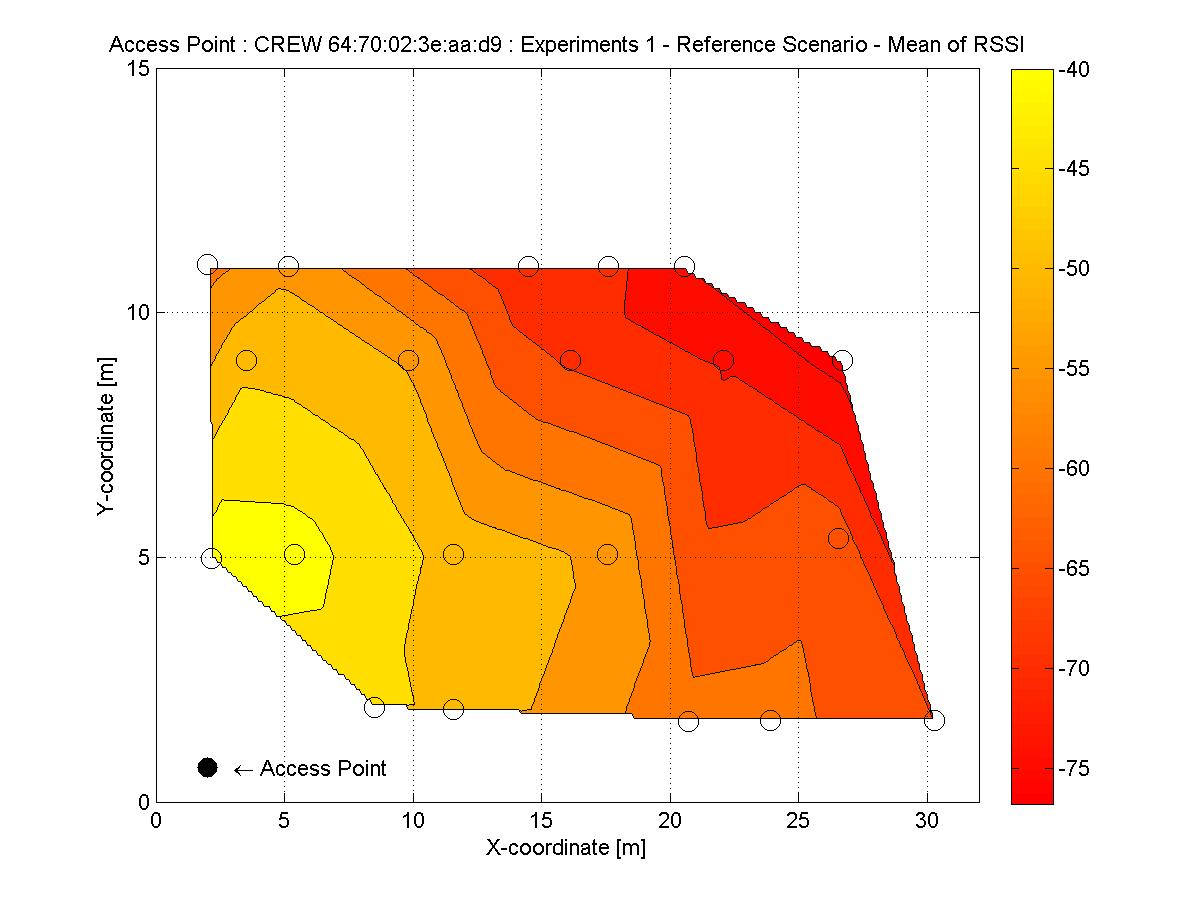
\includegraphics[width=13cm]{../../Source/plot/CREW_d9/d9_Ref_Ex_1_Mean.jpg} \\
	\includegraphics[width=13cm]{../../Source/plot/CREW_d9/d9_Ref_Ex_2_Mean.jpg} \\
	\includegraphics[width=13cm]{../../Source/plot/CREW_d9/d9_Ref_Ex_3_Mean.jpg} \\
	\includegraphics[width=13cm]{../../Source/plot/CREW_d9/d9_Ref_Ex_4_Mean.jpg} \\
	\includegraphics[width=13cm]{../../Source/plot/CREW_d9/d9_Ref_Ex_1_Variance.jpg} \\
	\includegraphics[width=13cm]{../../Source/plot/CREW_d9/d9_Ref_Ex_2_Variance.jpg} \\
	\includegraphics[width=13cm]{../../Source/plot/CREW_d9/d9_Ref_Ex_3_Variance.jpg} \\
	\includegraphics[width=13cm]{../../Source/plot/CREW_d9/d9_Ref_Ex_4_Variance.jpg} 
\end{longtable}

\subsection{Interference Scenario 1} 
Following plots show mean and variance of RSSI values from the access point (CREW 64:70:02:3e:aa:d9). Mean and Variance are plotted spatially with color map to show the significance. As described in the section \ref{scene:int:1}, these experiments were conducted in a scenario where IEEE 802.11 channel was jammed with the maximum transmission power using signal generators.
\begin{longtable}
	{lr} 
	\includegraphics[width=13cm]{../../Source/plot/CREW_d9/d9_Sig_Ex_1_Mean.jpg} \\
	\includegraphics[width=13cm]{../../Source/plot/CREW_d9/d9_Sig_Ex_2_Mean.jpg} \\
	\includegraphics[width=13cm]{../../Source/plot/CREW_d9/d9_Sig_Ex_1_Variance.jpg} \\
	\includegraphics[width=13cm]{../../Source/plot/CREW_d9/d9_Sig_Ex_2_Variance.jpg} \\
\end{longtable}

\subsection{Interference Scenario 2} 
Following plots show mean and variance of RSSI values from the access point (CREW 64:70:02:3e:aa:d9). Mean and Variance are plotted spatially with color map to show the significance. As described in the section \ref{scene:int:2}, these experiments were conducted in a scenario where interference is caused by Wifi data traffic between a server and email client, data client and video client.
\begin{longtable}
	{lr} 
	\includegraphics[width=13cm]{../../Source/plot/CREW_d9/d9_Wifi_Ex_1_Mean.jpg} \\
	\includegraphics[width=13cm]{../../Source/plot/CREW_d9/d9_Wifi_Ex_2_Mean.jpg} \\
	\includegraphics[width=13cm]{../../Source/plot/CREW_d9/d9_Wifi_Ex_1_Variance.jpg} \\
	\includegraphics[width=13cm]{../../Source/plot/CREW_d9/d9_Wifi_Ex_2_Variance.jpg} \\
\end{longtable}

\subsection{Group Variances} 
Following plots show group variances of RSSI values from the access point (CREW 64:70:02:3e:aa:d9) of experiments with reference scenario, interference scenario 1 and interference scenario 2. As described in the section \ref{sec:repeat}, Group variances are calculated.  
\begin{longtable}
	{lr} 
	\includegraphics[width=13cm]{../../Source/plot/CREW_d9/d9_Ref_Group_Variance.jpg} \\
	\includegraphics[width=13cm]{../../Source/plot/CREW_d9/d9_Sig_Group_Variance.jpg} \\
	\includegraphics[width=13cm]{../../Source/plot/CREW_d9/d9_Wifi_Group_Variance.jpg} \\
\end{longtable}
\section{Access Point : CREW 64:70:02:3e:aa:ef} 
The details of the access point are given below.
\begin{itemize}
	\item SSID : CREW 
	\item BSSID : 64:70:02:3e:aa:ef 
	\item Location : X-axis - 4.0m, Y-axis - 14.8m 
	\item Frequency : 2.4 GHz 
\end{itemize}
\subsection{Reference Scenario} 
Following plots show mean and variance of RSSI values from the access point (CREW 64:70:02:3e:aa:ef). Mean and Variance are plotted spatially with color map to show the significance. As described in the section \ref{scene:ref}, these experiments were conducted in a scenario where no artificial interference is generated and the presence of uncontrolled interference is minimized.
\begin{longtable}
	{lr} 
	\includegraphics[width=13cm]{../../Source/plot/CREW_ef/ef_Ref_Ex_1_Mean.jpg} \\
	\includegraphics[width=13cm]{../../Source/plot/CREW_ef/ef_Ref_Ex_2_Mean.jpg} \\
	\includegraphics[width=13cm]{../../Source/plot/CREW_ef/ef_Ref_Ex_3_Mean.jpg} \\
	\includegraphics[width=13cm]{../../Source/plot/CREW_ef/ef_Ref_Ex_4_Mean.jpg} \\
	\includegraphics[width=13cm]{../../Source/plot/CREW_ef/ef_Ref_Ex_1_Variance.jpg} \\
	\includegraphics[width=13cm]{../../Source/plot/CREW_ef/ef_Ref_Ex_2_Variance.jpg} \\
	\includegraphics[width=13cm]{../../Source/plot/CREW_ef/ef_Ref_Ex_3_Variance.jpg} \\
	\includegraphics[width=13cm]{../../Source/plot/CREW_ef/ef_Ref_Ex_4_Variance.jpg} 
\end{longtable}

\subsection{Interference Scenario 1} 
Following plots show mean and variance of RSSI values from the access point (CREW 64:70:02:3e:aa:ef). Mean and Variance are plotted spatially with color map to show the significance. As described in the section \ref{scene:int:1}, these experiments were conducted in a scenario where IEEE 802.11 channel was jammed with the maximum transmission power using signal generators.
\begin{longtable}
	{lr} 
	\includegraphics[width=13cm]{../../Source/plot/CREW_ef/ef_Sig_Ex_1_Mean.jpg} \\
	\includegraphics[width=13cm]{../../Source/plot/CREW_ef/ef_Sig_Ex_2_Mean.jpg} \\
	\includegraphics[width=13cm]{../../Source/plot/CREW_ef/ef_Sig_Ex_1_Variance.jpg} \\
	\includegraphics[width=13cm]{../../Source/plot/CREW_ef/ef_Sig_Ex_2_Variance.jpg} \\
\end{longtable}

\subsection{Interference Scenario 2} 
Following plots show mean and variance of RSSI values from the access point (CREW 64:70:02:3e:aa:ef). Mean and Variance are plotted spatially with color map to show the significance. As described in the section \ref{scene:int:2}, these experiments were conducted in a scenario where interference is caused by Wifi data traffic between a server and email client, data client and video client.
\begin{longtable}
	{lr} 
	\includegraphics[width=13cm]{../../Source/plot/CREW_ef/ef_Wifi_Ex_1_Mean.jpg} \\
	\includegraphics[width=13cm]{../../Source/plot/CREW_ef/ef_Wifi_Ex_2_Mean.jpg} \\
	\includegraphics[width=13cm]{../../Source/plot/CREW_ef/ef_Wifi_Ex_1_Variance.jpg} \\
	\includegraphics[width=13cm]{../../Source/plot/CREW_ef/ef_Wifi_Ex_2_Variance.jpg} \\
\end{longtable}

\subsection{Group Variances} 
Following plots show group variances of RSSI values from the access point (CREW 64:70:02:3e:aa:ef) of experiments with reference scenario, interference scenario 1 and interference scenario 2. As described in the section \ref{sec:repeat}, Group variances are calculated.  
\begin{longtable}
	{lr} 
	\includegraphics[width=13cm]{../../Source/plot/CREW_ef/ef_Ref_Group_Variance.jpg} \\
	\includegraphics[width=13cm]{../../Source/plot/CREW_ef/ef_Sig_Group_Variance.jpg} \\
	\includegraphics[width=13cm]{../../Source/plot/CREW_ef/ef_Wifi_Group_Variance.jpg} \\
\end{longtable}

% ================================================================
% Conclusion
% ================================================================
\chapter{Conclusion and future work} In this work, we presented how we have done experiments with and without controlled interferences to study the variation of RSSI values. Experiments yielded a large amount of data sets that must be processed and analyzed. Therefore we have implemented a tool to visualize the raw data obtained from the experiments, so that we could see the data collected from any experiment, at any point of location in the testbed, grouped based on BSSID. Furthermore, this tool helped us to see statistical graph of the raw data. Furthermore, the data was studied and graphs were plotted to understand whether RSSI values change due to interferences. Finlay, we recommend to carry out more experiments to get a significant results with the help of the data retrieved in this project. 

\subsection*{Resources for future work}
Source code of the visualization and data analysis tool, scripts used to plot the results, tools, documents and data that was gathered during this project is available in this online repository \url{https://github.com/AravinthPanch/rssi} for future work. 



% ================================================================
% Bibliography
% ================================================================
\begin{thebibliography}
	{1} \bibitem{ref:wifi} IEEE Std 802.11-2007: "Part 11: Wireless LAN Medium Access Control (MAC) and Physical Layer (PHY) Specifications", IEEE, New York, NY, USA, 1999-2007. \bibitem{ref:randr} Koji Horie, Yusuke Tsutsumi, Yukio Takao, Tomomichi Suzuki, "Calculation Of Repeatability And Reproducibility For Qualitative Data", Department of Industrial Administration, Tokyo University of Science. \bibitem{ref:randr2} Damir Markucic, "How to determine repeatability and reproducibility", 3rd European-American Workshop on NDE Reliability, Department of Quality, University of Zagreb. \bibitem{ref:wifi:chipset} Lui, Gough, et al: "Differences in RSSI Readings made by Different Wi-Fi Chipsets: A Limitation of WLAN Localization", Localization and GNSS (ICL-GNSS), 2011 International Conference on. IEEE, 2011. \bibitem{ref:wireless} Lee, Jin-Shyan, Yu-Wei Su, and Chung-Chou Shen et al: "A Comparative Study of Wireless Protocols: Bluetooth, UWB, ZigBee, and Wi-Fi", Industrial Electronics Society, 2007. IECON 2007. 33rd Annual Conference of the IEEE. IEEE, 2007. \bibitem{ref:rssi} Parameswaran, Ambili Thottam; Husain, M, I.; Upadhyaya, S. "Is RSSI a Reliable Parameter in Sensor Localization Algorithms – An Experimental Study". September 2009. 28th International Symposium On Reliable Distributed Systems, New York. Retrieved 17 March 2013. \bibitem{ref:evarilos} EVARILOS Project, "Evaluation Of Rf Based Indoor Localization Solutions For The Future internet". \bibitem{ref:crew} CREW Project, "Cognitive Radio Experimentation World". \bibitem{ref:twist} TWIST Testbed, "TKN Wireless Indoor Sensor network Testbed". 
\end{thebibliography}

% ================================================================
% Data
% ================================================================
\chapter{Appendix} 
\section{Access Point : CREW 64:70:02:3e:9f:63} 
\subsection{Variance, Mean, Group Variance of Reference Scenario} 
\begin{longtable}
	{lr} 
	\includegraphics[width=15cm]{../../Source/plot/data/63_ref1.png} \\
	\includegraphics[width=15cm]{../../Source/plot/data/63_ref2.png} \\
\end{longtable}
\subsection{Variance, Mean, Group Variance of Interference Scenario 1} 
\includegraphics[width=15cm]{../../Source/plot/data/63_int1.png} 
\subsection{Variance, Mean, Group Variance of Interference Scenario 2} 
\includegraphics[width=15cm]{../../Source/plot/data/63_int2.png} 

\pagebreak 
\section{Access Point : CREW 64:70:02:3e:aa:11} 
\subsection{Variance, Mean, Group Variance of Reference Scenario} 
\begin{longtable}
	{lr} 
	\includegraphics[width=15cm]{../../Source/plot/data/11_ref1.png} \\
	\includegraphics[width=15cm]{../../Source/plot/data/11_ref2.png} \\
\end{longtable}
\subsection{Variance, Mean, Group Variance of Interference Scenario 1} 
\includegraphics[width=15cm]{../../Source/plot/data/11_int1.png} 
\subsection{Variance, Mean, Group Variance of Interference Scenario 2} 
\includegraphics[width=15cm]{../../Source/plot/data/11_int2.png}

\pagebreak 
\section{Access Point : CREW 64:70:02:3e:aa:d9} 
\subsection{Variance, Mean, Group Variance of Reference Scenario} 
\begin{longtable}
	{lr} 
	\includegraphics[width=15cm]{../../Source/plot/data/d9_ref1.png} \\
	\includegraphics[width=15cm]{../../Source/plot/data/d9_ref2.png} \\
\end{longtable}
\subsection{Variance, Mean, Group Variance of Interference Scenario 1} 
\includegraphics[width=15cm]{../../Source/plot/data/d9_int1.png} 
\subsection{Variance, Mean, Group Variance of Interference Scenario 2} 
\includegraphics[width=15cm]{../../Source/plot/data/d9_int2.png}

\pagebreak 
\section{Access Point : CREW 64:70:02:3e:aa:ef} 
\subsection{Variance, Mean, Group Variance of Reference Scenario} 
\begin{longtable}
	{lr} 
	\includegraphics[width=15cm]{../../Source/plot/data/ef_ref1.png} \\
	\includegraphics[width=15cm]{../../Source/plot/data/ef_ref2.png} \\
\end{longtable}
\subsection{Variance, Mean, Group Variance of Interference Scenario 1} 
\includegraphics[width=15cm]{../../Source/plot/data/ef_int1.png} 
\subsection{Variance, Mean, Group Variance of Interference Scenario 2} 
\includegraphics[width=15cm]{../../Source/plot/data/ef_int2.png}

% ================================================================
% End of Document
% ================================================================
\end{document} 
